\documentclass[12pt]{article}

\usepackage{pgfplots}
\pgfplotsset{compat=1.18} % Or adjust depending on your TeX distribution
\usepackage[utf8]{inputenc}	% Para caracteres en español
\usepackage{amsmath,amsthm,amsfonts,amssymb,amscd}
\usepackage{multirow,booktabs}
\usepackage[table]{xcolor}
\usepackage{fullpage}
\usepackage{lastpage}
\usepackage{newtxtext}
\usepackage{newtxmath}
\usepackage{enumitem}
\usepackage{fancyhdr}
\usepackage{mathrsfs}
\usepackage{wrapfig}
\usepackage{setspace}
\usepackage{calc}
\usepackage{multicol}
\usepackage{cancel}
\usepackage[retainorgcmds]{IEEEtrantools}
\usepackage[margin=3cm]{geometry}
\usepackage{amsmath}
\newlength{\tabcont}
\setlength{\parindent}{0.0in}
\setlength{\parskip}{0.05in}
\usepackage{empheq}
\usepackage{framed}
\usepackage[most]{tcolorbox}
\usepackage{xcolor}
\colorlet{shadecolor}{orange!15}
\parindent 0in
\parskip 12pt
\geometry{margin=1in, headsep=0.25in}
\theoremstyle{definition}
\newtheorem{defn}{Definition}
\newtheorem{reg}{Rule}
\newtheorem{exer}{Exercise}
\newtheorem{note}{Note}
\newtheorem{theorem}{Theorem}
\setcounter{section}{0}
\usepackage{chngcntr}
\usepackage{hyperref}
\counterwithin*{equation}{section}
\counterwithin*{equation}{subsection}

\begin{document}

\url{https://famaf.aulavirtual.unc.edu.ar/course/view.php?id=254}

\section{Taylor}

Let $f \in C^n[a, b]$ and assume $f^{(n+1)}$ exists in $(a, b)$. Then 
for any $c, x \in [a, b]$ there is some $\zeta$ between $c$ and $x$ s.t. 

\begin{equation}
f(x) = \sum_{k=0}^{n} \frac{f^{(k)}(c)(x-c)^k}{k!} + E_n(x)
\end{equation}

where 

\begin{equation*}
    E_n(x) = \frac{f^{(n+1)}(\zeta)(x-c)^{n+1}}{(n+1)!}
\end{equation*}

Equation $(1)$ is called the Taylor expansion of $f$ around $c$. 

\begin{shaded}
    \textbf{Observation.} The famous \textit{mean value theorem} is simply the
    case $n = 0$ of Taylor's expansion: if $f \in C[a, b]$ and $f'$ exists on
    $(a, b)$, then for $x, c \in [a, b]$

    \begin{equation*}
        f(x) = f(c) + f'(\zeta)(x-c)
    \end{equation*}

    where $\zeta$ is between $c$ and $x$. Take $x=b, c = a$ and the theorem
    appears:

    \begin{equation*}
        f(b) - f(a) = f'(\zeta)(b-a)
    \end{equation*}
\end{shaded}

We typically extend the Taylor approximation of $f$ around a point $r$, where
$r = x + h$ is an approximation some value of interest $x$. This is useful
because said approximation gives 

\begin{equation*}
    f(r) = f(x+h) = f(x) + f'(x)h + \frac{ f^{''}(x) }{2}h^2 + \ldots + 
    \frac{ f^{(n)}(x) }{n!}h^n + E_n(h)
\end{equation*}

In other words, this strategy allows us to extend $f(r)$ in terms of $x$ and
$h$, the approximation and its error. Usually, $r, h$ are unknown but $h$ can be
bounded.

\pagebreak

\section{Alg. de Horner: Polynomial evaluation} 

Consider 

\begin{equation*}
    p(x) = \sum_{i=0}^n a_ix^i
\end{equation*}

We wish to compute $p(k)$ for a given $k \in \mathbb{R}$ minimizing the number
of operations. Directly computing $a_0 + a_1k_1 + \ldots$ leads to $n$ sums. The
$i$th term requires computing $k^i$, which means $i$ product operations, for a
totall of $\sum_{i=1}^n i = \frac{n(n+1)}{2}$ products.  The total number of
operations is then 

\begin{equation*}
    \Theta = n + n(n+1) / 2
\end{equation*}

The associated complexity is $\mathcal{O}(n^2)$. 

Horner's method consists of re-writing $p(x)$ so that the number of products is
reduced. One writes 

\begin{equation*}
    p(x) = a_0 + x b_0
\end{equation*}

where $b_{n-1} = a_n$ and for $0 \leq i < n - 1$:

\begin{equation*}
    b_{i-1} = a_{i} + xb_{i}
\end{equation*}

\begin{shaded}
    \begin{example}
        \normalfont
        Let $p(x) = 3 + 5x -4x^2 + 0x^3 + 6x^4$, giving $n = 4$. Then 
        $b_{3} = 6$ and 

        \begin{align*}
            &b_2 = a_3 + xb_3 = 6x,  &b_1 = a_2 + xb_2 = -4 + x(6x),\\
            &b_0 = a_1 + xb_1 = 5 + x(-4+x(6x)) 
        \end{align*}

        This finally gives

        \begin{equation*}
            p(x) = 3 + xb_0 = 3+x(5 +
            x(-4+x(6x)))
        \end{equation*}
    \end{example}
\end{shaded}

Here, one must perform $n$ sums again but only $n$ products. Thus, there are
$\Theta = n + n = 2n$ operations, giving a complexity of $\mathcal{O}(n)$ (in
the operation space). See the algorithm below:

\begin{align*}
&\textbf{input } n; a_i, i = 0, \ldots, n; x \\ 
& b_{n-1} \leftarrow a_n \\ 
& \textbf{for } i = n - 2 \textbf{ to } i = 0 \\ 
&\qquad b_{i} = a_{i+1} + x * b_{i+1} \\ 
&\textbf{od}\\
&y \leftarrow a_0 + x*b_0 \\ 
&\textbf{return } y
\end{align*}

It is easy to see in this code that the $\textbf{for}$ loop performs $n-1$
iterations, in each of which a single sum and a single product are computed. The
$n$th sum and $n$th product are performed in the computation of $y$, the final
result. 

A more polished version includes the last computatoin (the one in the assignment
of $y$) within the loop and makes no use of indexes:


\begin{align*}
&\textbf{input } n; a_i, i = 0, \ldots, n; x \\ 
& b \leftarrow a_n \\ 
& \textbf{for } i = n - 2 \textbf{ to } i = -1 \\ 
&\qquad b = a_{i+1} + x * b \\ 
&\textbf{od}\\
&\textbf{return } b
\end{align*}
 
In Python,


\small
\begin{quote}


\begin{verbatim}
def horner(coefs, x):
  n = len(coefs)-1
  b = coefs[n]

  for i in reversed(range(-1, n-1)):
    b = coefs[i+1] + x*b

  return b

\end{verbatim}

\end{quote}
\normalsize


It is trivial to adapt the code so that it returns the coefficients $b_0,
\ldots, b_{n-1}$ and not the final result, if needed.

\pagebreak 

\section{Error}

Let $r, \overline{r}$ be two real numbers s.t. the latter is an approximation of
the first. We define the \textbf{error} of the approximation to be $r -
\hat{r}$, and 

\begin{align*}
    \Delta r = \left| r - \overline{r} \right|, \qquad \delta r = \frac{\Delta
    r}{\left| r \right| }
\end{align*}

With $r$ unknown the strategy is to work with a known bound of $r$.

\pagebreak 

\section{Non-linear equations}

The general problem is to find members of the set $\mathcal{R}_f$ of roots of $f
\in \mathbb{R} \to \mathbb{R}$. The numerical strategy is to iteratively
approximate some $r \in \mathcal{R}_f$ until some pre-established threshold in
the error of approximation is met. 

More formally, the numerical strategy produces a sequence $\left\{ x_k
\right\}_{k\in \mathbb{N}}
$ which satisfies 

\begin{itemize}
    \item $\lim_{k\to \infty} \left\{ x_k \right\} = r$  for some $r \in
        \mathcal{R}_f$ 
    \item Either $e(x_k) < e(x_{k-1})$ or, more strongly, $\lim_{k\to \infty}
        e(x_k) = 0$, where $e(x_k)$ is some appropriate measure of the error of
        approximation.
\end{itemize}

\subsection{Bisection}

A very simple procedure: if a root exists in $[a, b]$, it iteratively shrinks
$[a,b]$ in halves (keeping the halves which contain the root) until the interval
is of sufficiently small length or the root is found.

\begin{theorem}[Intermediate value]
    If $f$ is continuous in $[a, b]$ and $f(a)f(b) < 0$, then $\exists r \in
    \mathcal{R}_f$ s.t. $r \in [a, b]$.
\end{theorem}

Assume $f$ is continuous. A root exists in $[a, b]$ if $f(a)f(b) < 0$
(\textbf{Theorem 1}). If that is the case, the midpoint $(a+b) / 2$ is taken as
the approximation $x_0$. It is also trivial to observe that $x_0$ is \textit{at
most} at a distance of $(b-a) / 2$ from the real root, so $e_0 = |x_0 - r| \leq
(b-a) / 2$. 

If $f(x_0) = 0$ the procedure must end because a root was found. Otherwise,
sufficies to find which half of the interval contains a root computing
$f(a)f(c)$ and, if needed, $f(c)f(b)$.

The iterations may stop after reaching a maximum number of steps, when $|f(c)|$
is sufficiently close to zero, or when the error bound $|e_k| \leq (b_k - a_k) /
2$ (where $[a_k, b_k]$ is the interval of this iteration) is sufficiently small.

\begin{shaded}
    \textbf{(!)} The algorithm not always converges. Take $f(x) = 1 / x$. Clearly, it has no
    root. Yet setting $a = -1, b=1$ in the initial iteration falsely passes the
    test. (The problem obviously is that $f$ is not continuous in $[-1, 1]$.) If
    one sets
\end{shaded}

\pagebreak 

\begin{align*}
&\textbf{Input}: a, b, \delta, M, f\\  
&\textbf{Output}: \text{Tupla de la forma: } (r, \text{cota de error})\\
&f_a \leftarrow  f(a) \\ 
&f_b \leftarrow f(b) \\ 
&\qquad\\
&\textbf{if } f_a*f_b > 0 \\ 
&\qquad \textbf{return } ?\\ 
&\textbf{fi}\\
&\qquad\\
&\textbf{for } i = 1 \textbf{ to } i = M \textbf{ do } \\ 
&\qquad c \leftarrow a + (b-a) / 2 \\ 
&\qquad f_c \leftarrow f(c) \\ 
&\qquad \textbf{if } f_c = 0 \textbf{ then } \\ 
&\qquad\qquad \textbf{ return } (c, 0) \\ 
&\qquad\textbf{fi}\\
&\qquad \epsilon = \frac{b - a}{2}\\
&\qquad \textbf{if } \epsilon < \delta \textbf{ then } \\ 
& \qquad\qquad \textbf{break}\\
&\qquad\textbf{fi}\\
&\qquad \textbf{if } f_a*f_c < 0 \textbf{ then } \\ 
&\qquad \qquad b \leftarrow c \\ 
&\qquad\qquad f_b = f(b)\\
&\qquad\textbf{else } \\ 
&\qquad\qquad a \leftarrow c \\ 
&\qquad\qquad f_a = f(a)\\
&\qquad\textbf{fi} \\ 
&\textbf{od}\\
&\textbf{return } (c, \epsilon)
\end{align*}

\pagebreak 


\small
\begin{quote}

\begin{verbatim}
def bisection(f : callable, a : float, b : float, delta : float, M : int):

  s, e = f(a), f(b) # function values at (s)tart, (e)nd of interval

  if s*e > 0:
    raise ValueError("Interval [a, b] contains no root.")

  for i in range(M):

    c = a + (b-a)/2 
    m = f(c) # value of f at (m)idpoint

    if m == 0:
      return c, 0

    e = (b-a)/2
    if e < delta:
      return c, e

    if s*m < 0:
      b = c 
      e = f(b)
    else:
      a = c 
      s = f(a)
    
  return c, e

\end{verbatim}

\end{quote}
\normalsize

\pagebreak

\begin{theorem}
    If $\left\{ [a_i, b_i] \right\}_{i=0}^\infty $ are the intervals generated
    by the bisection method on iterations $i = 0, 1, \ldots$, then:

    \begin{enumerate}
        \item $\lim_{n\to
    \infty} a_n = \lim_{n \to \infty} b_n$ is a member of $\mathcal{R}_f$.
     \item If $c_n = \frac{1}{2}(a_n + b_n), r = \lim_{n \to \infty} c_n $, then 
         $|r - c_n| \leq \frac{1}{2^{n+1}}(b_0 - a_0)$
    \end{enumerate}

\end{theorem}


\small
\begin{quote}

\textbf{Proof.} \textbf{(1)} It is clear that $a_i \leq a_{i+1}$ and $b_i \geq b_{i+1}$,
since the interval on each iteration shrinks in one direction. 

$\therefore a_n, b_n$ are monotonous. 

But clearly $a_n$ is bounded by $b_0$ and $b_n$ is bounded by $a_0$. 

$\therefore $ $a_n, b_n$ are monotonous and bounded. 

$\therefore $ Their limits exist.

It is also clear that the interval shrinks to half its size on each iteration: 

\begin{equation}
    b_n - a_n = \frac{1}{2} (b_{n-1} - a_{n-1}), \qquad n \geq 1
\end{equation}

By recurrence on $(1)$,

\begin{equation}
    b_n - a_n = \frac{1}{2^n}(b_0 - a_0), \qquad n \geq 0
\end{equation}

Then 

\begin{equation}
   \lim_{n \to \infty} a_n - \lim_{n \to \infty} b_n = \lim_{n \to \infty} (a_n - b_n) 
    = \lim_{n \to \infty}  \frac{1}{2^n}(b_0 - a_0) = 0
\end{equation}

$\therefore ~ \lim_{n \to \infty} a_n = \lim_{n \to \infty} b_n$.


Since the limit of $a_n, b_n$ exists and $f$ is by assumption continuous, the
composition limit theorem applies and:

\begin{align}
    &\lim_{n \to \infty} \left( f(a_n) \cdot f(b_n) \right) \nonumber
\\
    =& \lim_{n \to \infty}    f(a_n) \cdot \lim_{n \to \infty} f(b_n) &\left\{ \text{Product of limits} \right\}  \nonumber \\ 
    =& f\left( \lim_{n \to \infty} a_n
\right) \cdot f\left( \lim_{n \to \infty} b_n \right)  &\left\{
\text{Composition limit theorem} \right\} \nonumber \\ 
    =& \left[ f(r) \right]^2 &\left\{ r = \lim_{n \to \infty} a_n \right\} 
\end{align}

The invariant of the algorithm is $f(a_n)f(b_n) < 0$. But due to the last
result,

\begin{equation*}
    \lim_{n \to \infty} f(a_n)f(b_n) \leq 0 \iff [f(r)]^2 \leq 0 \iff f(r) = 0
\end{equation*}

$\therefore r = \lim_{n \to \infty} a_n = \lim_{n \to \infty} b_n$ is a root.

\textbf{(2)} Follows directly from result $(2)$

\begin{align*}
    \left| r - c_n \right|  &= \left| r - \frac{1}{2}(b_n - a_n) \right| \\ 
                            &\leq
    \left| \frac{1}{2}(b_n - a_n) \right| \\ 
&=\left| \frac{1}{2^{n+1}}(b_0 - a_0) \right| &\left\{ \text{Result }(2)
\right\} 
\end{align*}



\end{quote}
\normalsize

\pagebreak 

\subsection{Newton's method}


Assume $r \in \mathcal{R}_f$ and $r = x + h$, with $x$ an approximation of $r$
and $h$ its error. Assume $f''$ exists and is continuous in some $I$ around $x$
s.t. $r \in I$. What we explained on Taylor expansions around a point gives:

\begin{equation*}
    0 = f(r) = f(x + h) = f(x) + f'(x)h + \mathcal{O}(h^2)
\end{equation*}

If $x$ is sufficiently close to $r$, $h$ is small and $h^2$ even smaller, so
that $\mathcal{O}(h^2)$ is unconsiderable:

\begin{equation*}
    0 \approx f(x) + hf'(x)
\end{equation*}

Therefore, 

\begin{equation}
    h \approx - \frac{f(x)}{f'(x)}
\end{equation}

From this follows that $r = x + h$ is approximated by 

\begin{equation*}
    r \approx x - \frac{f(x)}{f'(x)}
\end{equation*}

Since the approximation in $(5)$ truncated the terms of $\mathcal{O}(h^2)$
complexity, this new approximation is closer to $r$ than $x$ originally was. In
other words, $x - f(x) / f'(x)$ is a better approximation to $r$ than $x$
itself. 

Thus, if $x_0$ is an original approximation, we can define 

\begin{equation}
    x_{n+1} = x_n - \frac{f(x_n)}{f'(x_n)}
\end{equation}

to produce a sequence of approximations. This is the fundamental idea of
Newton's method.

\begin{align*}
&\textbf{Input: } x_0, M, \delta, \epsilon; \\ 
&v \leftarrow f(x_0) \\ 
&\textbf{if } |v| < \epsilon \textbf{ then return }  x_0 \textbf{ fi }\\ 
&\textbf{for } k = 1 \textbf{ to } k = M \textbf{ do } \\ 
&\qquad x_1 \leftarrow x_0 - \frac{v}{f'(x_0)} \\
&\qquad v \leftarrow f(x_1) \\ 
&\qquad \textbf{if } \left| x_1 - x_0 \right| < \delta \lor v < \epsilon
\textbf{ then } \\ 
&\qquad\qquad \textbf{return } x_1 \\ 
&\qquad\textbf{fi} \\ 
&\qquad x_0 \leftarrow x_1 \\ 
&\textbf{od} \\ 
&\textbf{return } x_0
\end{align*}

The predicate $\left| x_1 - x_0 \right| < \delta$ checks whether our algorithm
is adjusting $x$ in a negligible degree. If that is the case, we
should stop. 

\begin{theorem}
    If $f''$ continuous around $r \in \mathcal{R}_f$ and $f'(r) \neq 0$, then
    there is some $\delta > 0$ s.t. if $\left| r - x_0 \right| \leq \delta $,
    then: 

    \begin{itemize}
        \item $\left| r - x_n \right| \leq \delta $ for all $n \geq 1$. 
        \item $\left\{ x_n \right\} $ converges to $r$  
        \item The convergence is quadratic, i.e. there is a constant $c(\delta)$
            and a natural $N$ s.t. $\left| r - x_{n+1} \right| \leq c\left| r -
            x_n\right|^2  $ for all $n \geq N$.
    \end{itemize}

\end{theorem}



\small
\begin{quote}

\textbf{Proof.} Let $e_n = r - x_n$ be the error in the $n$th approximation. Assume $f''$ is
continuous and $f(r) = 0$, $f'(r) \neq 0$. Then 

\begin{align}
    e_{n+1} &= r-  x_{n+1}  \nonumber \\ 
&= r - \left( x_n - \frac{f(x_n)}{f'(x_n)} \right) \nonumber \\ 
&= r - x_n  + \frac{f(x_n)}{f'(x_n)}\nonumber \\
&=\frac{e_n f'(x_n) + f(x_n)}{f'(x_n)}
\end{align}

Thus, the error at any given iteration is a function of the error at the
previous iteration. Now consider the expansion of $f(r)$ as 

\begin{equation}
    f(r) = f(x_n - e_n) = f(x_n) + e_nf'(x_n) + \frac{e_n^2f''(\zeta_n)}{2}
\end{equation}

for $\zeta_n$ between $x_n$ and $r$. This equation gives 

\begin{equation}
    e_n f'(x_n) + f(x_n) = -\frac{1}{2} f''(\zeta_n)e_n^2
\end{equation}

The expression in $(5)$ is the numerator in $(3)$, whereby we obtain via
substitution: 

\begin{equation}
    e_{n+1} =  -\frac{1}{2}\frac{f''(\zeta_n)e^2_n}{f'(x_n)} 
\end{equation}

Equation $(6)$ ensures that the error scales quadratically. Now we wish to
bound the error expression in $(6)$. To bound $e_{n+1}$, we take
$\delta > 0$ to define a neighbourhood of length $\delta$ around $r$. For any
$x$ in this neighbourhood, $(6)$ reaches its maximum when the numerator is
maximized and the denominator is minimized:

\begin{equation*}
    c(\delta) = \frac{1}{2} \frac{ \max_{\left| x - r \right| \leq \delta }
    \left| f''(x) \right|  }{\min_{\left| x-r \right| \leq \delta \left| f'(x) \right|  }}
\end{equation*}

In other words, $c(\delta)$ is the maximum value which $e_{n+1}$ can take if
$\zeta_n, x_n$ are assumed to belong to the neighbourhood. Now we make two
assumptions: 

\begin{enumerate}
    \item $x_0$ belongs to the neighbourhood, i.e. $\left| x_0 - r \right| \leq
        \delta$ 
    \item $\delta$ is sufficiently small so that $\varrho := \delta c(\delta) < 1$.
\end{enumerate}

Note that, since $\zeta_0$ is between $x_0$ and $r$, assumption (1) ensures that
$\zeta_0$ is also in the neighbourhood, i.e. $\left| r - \zeta_0 \right| \leq
\delta$. Then we have:

\begin{equation*}
    \left| e_0 \right| = \frac{1}{2} \left| f''(\zeta_0) / f'(x_0) \right| \leq c(\delta)
\end{equation*}

Then:

\begin{align*}
    \left| x_1 - r \right|  
    &= \left| e_1 \right|  \\ 
    &= \left| e_0^2 \cdot \frac{1}{2} f''(\zeta_0) / f'(x_0)  \right|  \\ 
    &\leq |e_0^2| c(\delta) &\left\{ \frac{1}{2}f''(\zeta_0) / f'(x_0) \leq c(\delta) \right\}  \\ 
    &\leq |e_0| \delta c(\delta) &\left\{ \left| e_0 \right| \leq \delta
    \right\}  \\ 
    &=\left| e_0 \right| \varrho &\left\{ \varrho = \delta c(\delta) \right\} \\
    &< \left| e_0 \right|  &\left\{ \varrho < 1 \right\}  \\ 
    &\leq \delta
\end{align*}

$\therefore $ $\left| e_1 \right| < \left| e_0 \right| \leq \delta$, which means
the error decreases. This argument may be repeated inductively, giving:
 
\begin{align*}
    &\left| e_1 \right|  \leq \varrho \left| e_0 \right|  \\ 
    &\left| e_2 \right|  \leq \varrho \left| e_1 \right| \leq \varrho^2 \left| e_0 \right|   \\ 
    &\left| e_3 \right|  \leq \varrho \left| e_2 \right| \leq \varrho^3 \left| e_0 \right|   \\ 
    &\vdots
\end{align*}

In general, $\left| e_{n} \right| \leq \varrho^n \left| e_0 \right|
$. And since $0 \leq \varrho < 1$, we have $\varrho^n \to 0$ when $n \to \infty$,
entailing that $\left| e_n \right| \to 0$ when $n \to \infty$.
\end{quote}
\normalsize

\begin{theorem}
    If $f''$ is continuous in $\mathbb{R}$, and if $f$ is increasing, convex,
    and has a root, then said root is unique and Newton's method converges to it
    from any starting point.
\end{theorem}

\begin{shaded}
    Recall that $f$ is convex if $f''(x) > 0$ for all $x$. Graphically, it is
    convex if the line connecting two arbitrary points of $f$ lies above the
    curve of $f$ between those two points.
\end{shaded}


\subsection{Secant method}

In Netwon's method, 

\begin{equation*}
    x_{n+1} = x_n - \frac{f(x_n)}{f'(x_n)}
\end{equation*}

The function of interest is $f$. We cannot escape computing $f(x_n)$, but it
would be desirable to avoid the computation of $f'(x_n)$, which may potentially
be expensive. Since

\begin{equation*}
    f'(x) = \lim_{h \to x}  \frac{f(x) - f(h)}{x-h}
\end{equation*}

it is natural to suggest 

\begin{equation}
    f'(x_n) \approx \frac{f(x_n) - f(x_{n-1})}{x_n - x_{n-1}}
\end{equation}

Graphically, this means we are not using the line tangent to the point $(x_n,
f(x_n))$ but the line secant to the points $(x_n, f(x_n)$ and $(x_{n-1},
f(x_{n-1}))$. The point $x_{n+1}$ is then the value of $x$ where this secant
line has a root.

\subsection{Fixed point iteration}

The key observation is  this: if $r \in \mathcal{R}_f$, then $g(x) = x - kf(x)$
has $r$ as fixed point, for any $k \in \mathbb{R}$. Inversely, if $g$ has a
fixed point in $r$, then $r \in \mathcal{R}_f$. 

\begin{theorem}
    (1) Let $g \in C[a, b]$ and assume $g(x) \in [a, b]$ for all $x \in [a, b]$.
    Then there is a  fixed point of $g$ in $[a, b]$.

    (2) If, on top of previous conditions, $g$ is differentiable in $(a, b)$ and
    there is some $k < 1$ s.t. $\left| g'(x) \right| \leq k$ for all $x \in
    (a,b)$, then the fixed point referred in (1) is unique.
\end{theorem}

\begin{shaded}
    \begin{theorem}[Mean value theorem]
        Let $f : [a, b] \to \mathbb{R}$ continuous and differentiable on $(a,
        b)$ with $a < b$. Then there is some $c \in (a, b)$  s.t. 

        \begin{equation*}
            f'(c) = \frac{ f(b) - f(a) }{b - a}
        \end{equation*}
    \end{theorem}

    The interpretation is simple: consider the line secant to $f$ on $a, b$. The
    theorem ensures that there is some point $c$ s.t. the line tangent to $c$ is
    parallelt to said secant (equal slopes).
\end{shaded}

\small
\begin{quote}

\textbf{Proof.} (1) If $a$ or $b$ are fixed points the proof is done so assume
otherwise. Since $g(x) \in [a, b]$,  we have $g(a) > a$ and $g(b) < b$.


Take $\varphi(x) = g(x) - x$, which is continuous and defined in $[a,
b]$. Then 

\begin{equation*}
    \varphi(a) = g(a) - a > 0, \qquad \varphi(b) = g(b) - b < 0
\end{equation*}

Then $\varphi(a)\varphi(b) < 0$. Then, by the intermediate value theorem,
$\varphi$ has a root in $(a, b)$. In otherwords, there is at least one $p$ s.t. 

\begin{equation*}
    \varphi(p) = g(p) - p = 0
\end{equation*}

$\therefore $ $g(p) = p$ is a fixed point of $g$.

(2) Assume two distinct fixed points $p, q$ exist in $[a, b]$. The mean value
theorem ensures the existence of some $\zeta$ between $p, q$ (and thus in $[a,
b]$) s.t.t 

\begin{equation}
    g'(\zeta) = \frac{g(a) - g(b)}{a - b} \iff g'(\zeta)(a-b) = g(a) - g(b)
\end{equation}

By hypothesis, $\left| g'(x) \right| \leq k < 1$. Since $p, q$ are assumed to
be fixed points, equation $(1)$ gives: 

\begin{align*}
    \left| p - q \right| 
    &= \left| g(p) - g(q) \right| \\ 
    &= \left| g'(\zeta) \right| \left| p - q \right|  \\ 
    &\leq k \left| p-q \right|  < \left| p - q \right| 
\end{align*}

But this is absurd. The contradiction arises from assuming $p, q$ to be
distinct. Therefore, the fixed point is unique.


\end{quote}
\normalsize

The fixed point algorithm begins with an approximation $p_0$. Then, 

\begin{equation*}
    p_n = g(p_{n-1})
\end{equation*}

If $g$ continuous and the sequence converges, then it converges to a fixed
point, since: 

\begin{equation*}
    p := \lim_{n \to \infty} p_n = \lim_{n \to \infty} g(p_{n-1}) = g\left(
    \lim_{n \to \infty} p_{n-1} \right) = g(p)
\end{equation*}

\begin{align*}
&\textbf{Input: } p, M, \delta \\ 
&p_{\text{previous}} = p\\
&\textbf{for } i = 1 \textbf{ to } i = M \textbf{ do } \\ 
&\qquad p \leftarrow g(p) \\ 
&\qquad \textbf{if } \left| p - p_{\text{previous}} \right| < \delta \textbf{ then } \\ 
&\qquad\qquad \textbf{return } p \\ 
&\qquad\textbf{fi}\\ 
&\qquad p_{\text{previous}} = p\\ 
&\textbf{od}\\ 
&\textbf{return }p
\end{align*}


\begin{theorem}
    Let $g \in C[a, b]$ be a self-map of $[a, b]$ differentiable in $(a, b)$.
    Assume there is a constant $0 < k < 1$ s.t. $\left| g'(x) \right| \leq k$
    for all $x \in (a, b)$.

    For all $p_0 \in [a, b]$, the sequence $p_n = g(p_{n-1})$ converges to the
    unique f ixed point $p$ in $(a, b)$.
\end{theorem}


\small
\begin{quote}

\textbf{Proof.} The mean value theorem ensures that 

\begin{align*}
    \left| p_n - p \right| 
    &= \left| g(p_{n-1}) - g(p) \right| \\ 
    &= |g'(\zeta_n)||(p_{n-1} - p)| \\ 
    &\leq k \left| p_{n-1} - p \right| 
\end{align*}

with $\zeta_n \in (a, b)$. More succintly, with $e_n := p_n - p$,

\begin{equation*}
    |e_n| \leq k \left| e_{n-1} \right| \leq k \left| e_{n-2} \right| \leq
    \ldots \leq k \left| e_0 \right| 
\end{equation*}

By recurrence,

\begin{equation*}
    \left| e_n \right| \leq k^n\left| e_0 \right| 
\end{equation*}

Since $0 < k < 1$, $k^n \to 0$ when $n \to \infty$, which entails $\left| e_n
\right| \to 0$ when $n \to \infty$. It follows that $\left\{ p_n \right\} \to
p$ when $n \to \infty$.

\end{quote}
\normalsize

Now let us consider the error of this method. Take $p_n = p + e_n$ and consider
the Taylor expanssion of $g$ around $p$ evaluated at $p_n = p+e_n$:

\begin{equation}
    g(p_n) = g(p + e_n) = \sum_{i=1}^{m-1} \frac{ g^{(i)}(p) }{i!} e_n^{i} +
    \frac{f^{(m)}(\zeta_n)}{(n+1)!} e_{n}^{m}
\end{equation}

See that in $(2)$, $n$ corresponds to the iteration we are dealing with, and
thus $\zeta_n$ and $e_n$ depend on it. On the contrary, $m$ is the degree to
which we expand the series of $g$ around $p$ evaluated at $p_n$. We also assume
that $\zeta_n$ lies between $p_n$ and $p$.

By definition, $g(p_n) = p_{n+1}$ so $(2)$ is nothing but an expression for this
value. Assume $g^{(k)}(p) = 0$ for $k = 1, 2, \ldots, m-1$, but $g^{(m)}(p) \neq
0$. Then 

\begin{align*}
    e_{n+1} 
    &= p_{n+1} - p\\ 
    &=g(p_n) - g(p) \\ 
    &=\frac{ g^{(m)}\left( \zeta_n \right)  }{m!}e_n^m 
\end{align*}

More succintly,

\begin{equation*}
    e_{n+1} = \frac{ g^{(m)}\left( \zeta_n \right)  }{m!}e_n^m 
\end{equation*}

Then 

\begin{equation*}
    \lim_{n \to \infty} \left| \frac{e_{n+1}}{e_n^m} \right|  = 
    \frac{\left| g^m(p) \right| }{m!}
\end{equation*}

which is a constant. In conclusion, if the derivatives of $g$ are null in $p$ up
to the order $m-1$, the method as an order of convergence of at least $m$. Three
results follow from this fact. 

\pagebreak 


\subsection{Exercises}

\begin{shaded}
    \textbf{(1)} Let $f(x) = (x+2)(x+1)^2 x(x-1)^3(x-2)$. To which root does
    the biscection method converge on the following intervals? 

    \begin{equation*}
        [-1.5, 2.5], \qquad [-0.5, 2.4], \qquad [-0.5, 3], \qquad [-3, -0.5]
    \end{equation*}
\end{shaded}

$(a)$ The midpoint of $I_0 = [-1.5, 2.5]$ is $c_0 := (2.5 - 1.5) / 2 = 1/2$. Since
$f(a)f(c) < 0$, we have $I_1 = [-1.5, 0.5]$. The midpoint of $I_1$ is $c_1 = -
0.5$, so $I_2$ will be $[-0.5, 0.5]$. The only root in this interval is $r = 0$,
so the algorithm converges to it.

$(b)$ The midpoint of $I_0 = [-0.5, 2.4]$ is $c := (2.4 - 0.5) / 2 = 0.95$. Then
$I_1 = [-1.5, 0.95]$. Same logic gives $c_1 = -0.725$ and then $I_2 = [-0.725,
0.95]$. The only root here is zero again. 

$(c, d)$ Same.

\pagebreak 

\begin{shaded}
    \textbf{(2)} We wish to find a root of $f$ in $[a, b]$ using bisection
    method and ensuring that the error is not greater than $\epsilon \in
    \mathbb{R}^+$. 

    $(a)$ Estimate the number of iterations sufficient to meet the criterion. 

    $(b)$ What is the number of iterations for $a = 0, b = 1, \epsilon =
    10^{-5}$? 
\end{shaded}

Let $e_n = x_n - r$. It is trivial to note that $\left| e_n \right| \leq
\frac{b_n - a_n}{2}$. Furthermore, the length of $I_1$ is half the length of
$I_0$, that of $I_2$ is half that of $I_1$, etc. In other words, 

\begin{equation*}
    \left| e_0 \right|  \leq \frac{b-a}{2}, \qquad \left| e_1 \right|  \leq
    \frac{b-a}{2^2}, \qquad \left| e_2 \right|  \leq
    \frac{b-a}{2^3}, \ldots
\end{equation*}

In general, 

\begin{equation*}
    \left| e_n \right|  \leq \frac{b-a}{2^{n+1}}
\end{equation*}

Imposing

\begin{equation*}
    \left| e_n \right|  \leq \frac{b-a}{2^{n+1}} \leq \epsilon
\end{equation*}

we satisfy our criterion, but we wish to express this bound in terms of $n$.
Now, clearly, 

\begin{align*}
&\frac{b-a}{2^{n+1}} \leq \epsilon  \\
\iff&\frac{ b-a }{\epsilon} \leq  2^{n+1} \\ 
\iff& \log_2\left( \frac{ b-a }{\epsilon} \right)  - 1 \leq n  \\
\impliedby& \log_2\left( \frac{b-a}{\epsilon} \right)  \leq n\\ 
\iff&\frac{ \ln \left( \frac{b-a}{\epsilon} \right)  }{\ln 2} \leq n
\end{align*}

which is our final answer. 

$(b)$ For $a = 0, b = 1, \epsilon = 10^{-5}$, we need 

\begin{equation*}
    n \geq \frac{\ln \left( \frac{1}{10^{-5}} \right) }{\ln 2} \approx 16.609
\end{equation*}

so $n = 17$ would suffice.

\pagebreak 

\begin{shaded}
    \textbf{(3)} Determine  graphically some root of $f(x) = 4\sin x + 1 - x$
    and perform three iterations of the bisection method to approximate. How
    many steps are needed to ensure an error less than $10^{-3}$?
\end{shaded}

Let us unveil the full power of LaTex:

\begin{center}
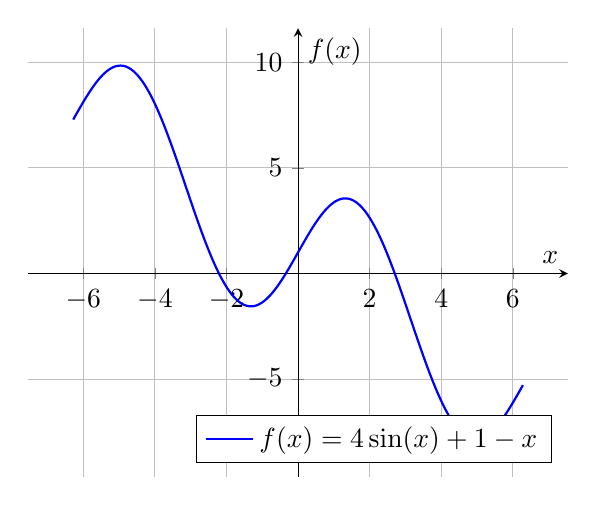
\begin{tikzpicture}
  \begin{axis}[
      axis lines=middle,
      xlabel={$x$},
      ylabel={$f(x)$},
      samples=200,
      domain=-2*pi:2*pi,
      grid=both,
      enlargelimits=true,
      legend pos=south east,
    ]
    \addplot[blue, thick] {4*sin(deg(x)) + 1 - x};
    \addlegendentry{$f(x) = 4\sin(x) + 1 - x$}
  \end{axis}
\end{tikzpicture}
\end{center}

I'm too lazy to perform the steps of the algorithm. The number of steps needed
again are given by 

\begin{equation*}
    n \geq \frac{\ln \left( \frac{4-2}{10^{-3}} \right) }{\ln 2} \approx 10.96
\end{equation*}

so taking $n = 11$ suffices.

\pagebreak 

\begin{shaded}
    \textbf{(4)} Let $a > 0$. Computing $\sqrt{a} $ is equivalent to finding the
    root of $f(x) = x^2 -  a$. 

    $(a)$ Show that Newton's sequence for this case is 

    \begin{equation*}
        x_{n+1} = \frac{1}{2}\left( x_n + \frac{a}{x_n} \right)  
    \end{equation*}

    $(b)$ Prove that f or any $x_0 > 0$, the approximations $\left\{ x_n
    \right\} $ satisfy $x_n \geq \sqrt{a} $ for $n \geq 1$. 

    $(c)$ Prove $\left\{ x_n \right\} $ is sdecreasing. 

    $(d)$ Conclude that the sequence converges to $\sqrt{a} $
\end{shaded}

$(a)$ In Newton's algorithm, 

\begin{equation*}
    x_{n+1} = x_n - \frac{f(x_n)}{f'(x_n)}
\end{equation*}

Clearly, 

\begin{equation*}
    f'(x) = \frac{d}{dx} (x^2 - a) = 2x
\end{equation*}

Therefore, 

\begin{align*}
    x_{n+1} 
    &= x_n - \frac{x_n^2 - a}{2x_n} \\ 
    &= x_n - \frac{1}{2}\left( x_n - \frac{a}{x_n} \right)  \\ 
    &= \frac{1}{2}x_n + \frac{1}{2} \frac{a}{x_n} \\ 
    &=\frac{1}{2}\left( x_n + \frac{a}{x_n} \right) \qquad \blacksquare
\end{align*}

$(b)$ Let $x_0 > 0$. Recall that, among all Pythagorean means, the arithmetic
mean is the greatest, asuming positively-valued vectors. In particular, it is
greater or equal to the geometric mean:

\begin{equation*}
    \frac{1}{N}\sum_{i=1}^n y_i \geq \sqrt[n]{\prod_{i=1}^n y_i} 
\end{equation*}

for any set of points $y_1, \ldots, y_n$ all positive. In particular, 

\begin{equation*}
    x_{n+1} = \frac{1}{2}\left( x_n + \frac{a}{x_n} \right) \geq \sqrt{x_n \frac{a}{x_n}}
    = \sqrt{a} \qquad \blacksquare
\end{equation*}

$(c)$  

\begin{align*}
&\frac{1}{2}\left( x_n + \frac{a}{x_n} \right) \leq x_n \\ 
\iff& x_n + \frac{a}{x_n} \leq 2x_n\\
\iff &\frac{a}{x_n} \leq x_n\\
\iff& a \leq x_n^2 \\ 
\iff& \sqrt{a} \leq x_n
\end{align*}

which is true due to point $(b)$.


$(d)$ Let $e_n = x_n - \sqrt{a} $. We have shown $\left\{ x_n \right\} $ to be
decreasing and bounded below by $\sqrt{a} $. Therefore, it converges to a limit
$L$ (with $L$ the infimum of $\left\{ x_n \right\} $). Then 

\begin{equation*}
    \lim_{n \to \infty} x_{n} = \frac{1}{2}\lim_{n \to \infty} \left( x_{n-1} +
    \frac{a}{x_{n-1}}\right) = \frac{1}{2}L + \frac{a}{2L}
\end{equation*}

This induces the equation 

\begin{align*}
    L = \frac{L}{2} + \frac{a}{2L} 
    &\iff \frac{L}{2} = \frac{a}{2L} \\ 
    &\iff L^2 = a\\
    &\iff L = \sqrt{a}  \qquad \blacksquare
\end{align*}

\pagebreak 

\begin{shaded}
    \textbf{(5)} Propose an iteration formula to approximate $\frac{1}{\sqrt{a}
    }$ , with $a > 0$, using Newton's method. Decide the number of iterations
    needed so that the relative error in the approximation is less than
    $10^{-4}$ when starting from $x_0 = 1$ and taking $a = 5$.
\end{shaded}

Error: $e_n = r - x_n$, quadratitc, i.e. $| r - x_{n+1}| \leq c |r - x_n|^2$.

($a$. Iteration formula) Let $a > 0$ and assume we wish to approximate $1 /
\sqrt{a} $. Let $\varphi = \frac{1}{a}$, so that $\frac{1}{\sqrt{a} } =
\sqrt{\varphi} $. We see that we can express the problem of finding the
reciprocal of a root in terms of a simple root.

We know from the previous exercise that the iteration formula for
$\sqrt{\varphi} $ is 

\begin{equation*}
    x_{n+1}=\frac{1}{2}\left( x_n + \frac{\varphi}{x_n} \right)  
\end{equation*}

Now take $x_{0} = 1$ and $a = 5$, so that
$\varphi = \frac{1}{5}$. The relative error of approximation on iteration $n$ is 

\begin{equation*}
    e_n = \frac{ \left| x_n - \frac{1}{\sqrt{5} } \right|  }{\sqrt{5} }
\end{equation*}

Brute-forcing allows us  to see that $x_0, x_1, x_2, x_3$ do not meet the criterion,
but 

\begin{equation*}
    x_4 = 0.4472137791286728 ~ (\text{ jaja } )
\end{equation*}

has $e_4 < 10^{-4}$.

\pagebreak 

\begin{shaded}
    \textbf{(6)} Propose an iteration formula for $\sqrt[3]{R} $ where $R > 0$. Plot the
    function to see where the procedure converges.
\end{shaded}
Observe that finding $\sqrt[3]{R}$ is equivalent to finding a root of $f(x) =
x^3 - R$. 

\begin{center}
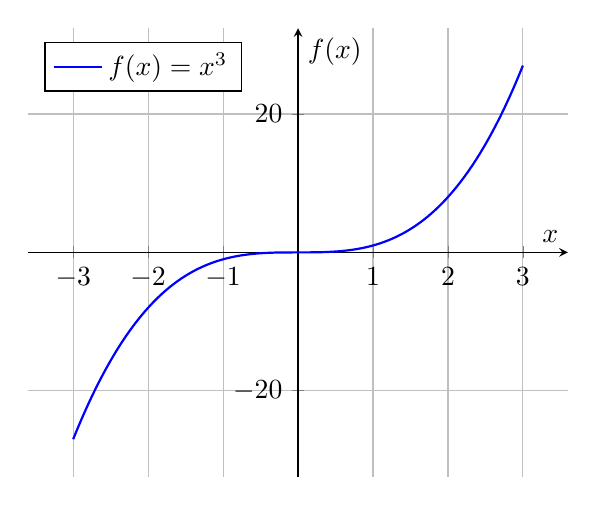
\begin{tikzpicture}
  \begin{axis}[
      axis lines=middle,
      xlabel={$x$},
      ylabel={$f(x)$},
      samples=200,
      domain=-3:3,
      grid=both,
      enlargelimits=true,
      legend pos=north west,
    ]
    \addplot[blue, thick] {x^3};
    \addlegendentry{$f(x) = x^3 $}
  \end{axis}
\end{tikzpicture}
\end{center}



But $f(x)$ is simply a vertical displacement of $x^3$, so $\frac{d}{dx} x^3 =
\frac{d}{dx} f(x)$ (which holds algebraically). In particular, the derivative
of $x^3$ approaches $0$ as $x \to 0$, meaning that Newton's method will fail to
converge for intervals of length $L$ around $0$ (with $L$ unspecified). The
graph suggests that an appropriate value for $L$ is $1$.

That said, since $\frac{d}{dx}f(x) = \frac{d}{dx} x^3$ (in other words, since
the derivative of the function is independent of $R$), and $\frac{d}{dx} x^3 =
3x^2$, we propose 

\begin{equation*}
    x_{n+1} = x_n - \frac{x_n^3}{3x_n^2} = x_n - \frac{x_n}{3} = \frac{2x_n}{3}
\end{equation*}

\pagebreak 

\begin{shaded}
    \textbf{(7)} $(a)$ Utilizando el teorema del valor intermedio, demostrar que $g(x)
    = \arctan(x) - \frac{2x}{1+x^2}$ tiene raíz $\alpha \in [1, \sqrt{3}] $. 

    $(b)$ Then show that if $\left\{ x_n \right\} $ is the sequence generated by
    Newton's method for $f(x) = \arctan(x)$, with $x_0 = \alpha$, it is the case 
    that $x_n = (-1)^n \alpha$.
\end{shaded}

$(a)$ It is known that $\arctan x$ is continuous in $\mathbb{R}$. Since $1 + x^2 >
0$ for all $x$, $2x / (1+x^2)$ is also continuous in $\mathbb{R}$. $\therefore $
$g$ is continuous in $\mathbb{R}$. And it is easy to verify as well that
$g(1)g(\sqrt{3} ) < 0$. 

$\therefore $ By virtue of the intermediate value theorem, there is a root
$\alpha$ of $g$ in $[1, \sqrt{3}] $.

$(b)$ Let $g_1(x) = \arctan x, g_2(x) = \frac{2x}{1+x^2}$, so that $g = g_1 -
g_2$. Since $\alpha > 0$, we have $g_1(\alpha) > 0, g_2(\alpha) > 0$. And since
$g(\alpha) = 0$ if and only if $g_1(\alpha) - g_2(\alpha) = 0$, we conclude that 
$g_1(\alpha) = g_2(\alpha)$. In other words, 

\begin{equation}
    \arctan \alpha = \frac{2\alpha}{1+\alpha^2}
\end{equation}

Since the derivative of $\arctan x$ is $1 / (1+x^2)$, equation $(1)$ may be
expressed as follows: 

\begin{equation}
    \arctan \alpha = 2\alpha \arctan'(\alpha)
\end{equation}

This entails that 

\begin{equation}
    \arctan' \alpha = \frac{\arctan \alpha}{2\alpha}
\end{equation}

Now take $x_0 = \alpha$ and consider Newton's sequence for $f(x) = \arctan x =
g_1(x)$. Clearly,

\begin{align*}
    x_1 
    &= \alpha - \frac{f(\alpha)}{f'(\alpha)} \\ 
    &= \alpha - \arctan \alpha \times \frac{2\alpha}{\arctan \alpha} &\left\{
    \text{Eq. } (3) \right\}  \\ 
    &= \alpha - 2\alpha \\ 
    &=-\alpha
\end{align*}

Same logic gives $x_2 = \alpha, x_3 = -\alpha, \ldots$ and the result should be
easy to generalize.

\pagebreak 

\begin{shaded}
    \textbf{(8)} Consider  for the fixed-point iteration the following
    functions, whose least positive root we wish to find:

    \begin{equation*}
        \phi(x) = x^3 - x - 1,\qquad \psi(x) = 2x - \tan x, \qquad \varphi(x) = \exp(-x) -
        \cos x
    \end{equation*}

    Find an iteration function and an interval which guarantees the method's
    convergence.
\end{shaded}

$(\phi)$ Let us analyize $\phi$ in order to
ascertain where its roots are. 

Consider that $\phi'(x) = 3x^2 - 1$, which means $\phi'$ has roots wherever
$3x^2 = 1$, which holds if and only if $x^2 = \frac{1}{3}$, or equivalently $x =
\pm \frac{\sqrt{3} }{3} $. Furthermore, $\phi'(x) < 0$ in the region $(-\sqrt{3}
/ 3, \sqrt{3}/3)  $ and $\phi'(x) > 0$ elsewhere. In conclusion, $\phi$ is
decreasing in $(-\sqrt{3} / 3, \sqrt{3} / 3)  $ and increasing everywhere else.

Now, observe that $\phi\left( \sqrt{3}/3  \right) < 0$. Combined with the fact
that $\phi$ is increasing in $(\sqrt{3} / 3, \infty)$, this means there is a
root of $\phi$ in this interval. (Note that $\phi$ is a polynomial without
asymptotic behavior.) Furthermore, $\phi \left( -\sqrt{3} / 3 \right)  < 0$. Again, this means there
is no root in $(\infty, \sqrt{3}  /3) $. 

$\therefore $ $\phi$ has one and only one root and it belongs to $(\sqrt{3} / 3,
\infty) $.

Now, suffices to note that $f(1.3)i < 0, f(1.4) > 0$, and the intermediate value
theorem ensures that there is a root in $(1.3, 1.4)$. $\therefore $ The only
root of $\phi$ lies within $(1.3, 1.4)$.

Now, we need only propose a function $f$ s.t. $r$ is a fixed-point of $f$ and 
$f(x) \in (1.3, 1.4)$ for all $x \in (1.3, 1.4)$. Consider that 

\begin{equation}
    \phi(x) = 0 \iff x^3 = x + 1 \iff x = \sqrt[3]{x+1} 
\end{equation}

So letting $f(x) := \sqrt[3]{x+1} $ ensures that the fixed point of $f$ is the
root of $\phi$. Furthermore, $f(1.3) \approx 1.32, f(1.4) \approx 1.33$. Now, 

\begin{equation*}
    f'(x) = \frac{1}{\sqrt[3]{(x+1)^2} }
\end{equation*}

Since $f'(x) > 0$ (as is simple to note), we know $f$ is increasing, which means
all $f(x) \in (1.32, 1.33)$ for $x \in [1.3, 1.4]$. Furthermore, 
$f'(x) \in (0, 1)$ and $f'(x)$ is clearly decreasing. This means that in $[1.3,
1.4]$, $f'$ has its maximum at $f'(1.4) \approx 0.573$. In other words, if we
let $k = 0.573$, we know $|g'(x)| = g'(x) < k$ for all $x \in [1.3, 1.4]$.

$\therefore $ $f$ is a self-map of $[1.3, 1.4]$, differentiable in $(1.3, 1.4)$,
and there is a constant $k \in (0, 1)$ s.t. $|g'(x)| < k$ for all $x \in (1.3,
1.4)$---where incidentally this constant is $g'(1.3)$. ]

$\therefore $ By virtue of \textbf{Theorem 7}, the fixed-point algorithm will
converge to the unique root $r \in (1.3, 1.4)$ if using the iteration function
$f(x) = \sqrt[3]{x+1} $ and the interval $[1.3, 1.4]$.

\pagebreak 

$(\psi)$ Let $\psi(x) = 2x - \tan x$. A root exists for $\psi(x)$ whenever 

\begin{equation*}
    x = \frac{\tan x}{2} = \frac{2 \sin x}{\cos x}
\end{equation*}

So we may define $g(x) := \tan x / 2$ guarantying that any fixed point of $g$ is
a root of $\psi$. Now, $\tan 0 = 0$ entails that $g(0) = 0$. 
Furthermore, $g(\pi / 4) = 1  /2$. Since $g'(x) = \sec^2(x) / 2$ is strictly
positive, $g$ is strictly increasing and this means for $x \in [0,
\frac{\pi}{4}]$ we have $g(x) \in [0, 1 / 2] \subseteq [0, \frac{\pi}{4}]$.

$\therefore $ $g$ is a self-map in $[0, \pi / 4]$.

$\therefore $ There is a fixed-point of $g$ in $[0, \pi / 4]$.

Consider now $g'(x) = \frac{1}{2}\sec^2(x)  = \frac{1}{2\cos^2 x}$. This is
clearly bounded in $(0, 1]$. To be more precise, it is geometrically obvious
that, for all $x \in [0, \pi / 4]$, $\sqrt{2} / 2 \leq \cos x \leq 1$, which
means $1/2 \leq \cos^2 x \leq 1$. In particular, $g'(x)$ reaches its maximum
when $\cos^2 x$ reaches its minimum, so $g'(x)$ reaches its maximum at $x =
\frac{\pi}{4}$: 

\begin{equation*}
    g'(\pi / 4) = \frac{1}{2\cos^2 \frac{\pi}{4}} = \frac{1}{2 \cdot 1 / 2} = 1
\end{equation*}

It follows that there is some constant $k \in (0, 1)$ such that $|g'(x)| \leq k$
for all $x \in (0, \pi / 4)$.

$\therefore $ There is a unique fixed point of $g$ in $[0, \pi / 4]$.

$\therefore $ There is a unique root of $\psi(x)$ in $[0, \pi / 4]$ and the
iteration method converges to it using this interval and the iteration function
$g$.


\pagebreak 

$(\varphi)$ Consider $\varphi(x) = \exp(-x) - \cos x$. This function is zero if
and only if $e^{-x} = \cos x$, which may be expressed as $x = -\ln \left( \cos x
\right) $. In other words, the roots of $\varphi$ correspond to the fixed points
of $f(x) = - \ln(\cos x)$. 

Now, $-1 \leq \cos x \leq 1$ but $\ln$ is defined only in $\mathbb{R}^+$. From
this follows that $f$ is defined only when $\cos x > 0$, i.e. in the right-hand
half of the unite circle. This corresponds to values of $x$ in $[0, \pi / 2)$ or 
$(3\pi / 2, 2\pi]$ (extended by any factor $2\pi k$, $k \in \mathbb{Z}$).

Take $I := [0, \pi /4] \subseteq \text{Dom}(f)$. See that $f(0) = -\ln(1) = 0$
and $f(\pi / 4) = -\ln(\sqrt{2} / 2 ) \approx 0.346 < \pi /4$. Furthermore, with
$u = \cos x$,

\begin{align*}
    \frac{df}{dx} = -\frac{d}{du} \ln(u) \times \frac{d}{dx} \cos x =
    \frac{\sin x}{\cos x} = \tan x
\end{align*}

which is strictly positive in $[0, \pi / 4]$. This suffices to prove that $f(x)
\in [0, \pi / 4]$ for all $x \in  [0, \pi / 4]$. 

$\therefore $ $f$ is a self-map of $[0, \pi / 4]$.

$\therefore $ There is a fixed point of $f$ in $[0, \pi / 4]$.

Now, $\tan x$ is increasing in $[0, \pi / 4]$ and, in particular, $\tan 0 = 0,
\tan \frac{\pi}{4} = 1$. This suffices to show that $|g'(x)| < 1$ for all $x \in
(0, \pi / 4)$. 

$\therefore $ There is a unique fixed point of $f$ in $[0, \pi / 4]$ and the
fixed point iteration algorithm converges to it when starting from said interval
with $f$ as iteration function.

\pagebreak 

\begin{shaded}
    \textbf{(10)} Let $x_{n+1} = 2^{x_n - 1}$ the formula used to solve $2x =
    2^x$. What interval should be chosen to ensure $\left\{ x_n \right\} $ is
    convergent? Calculate its limit.
\end{shaded}

The fixed-point algorithm uses the formula $p_n = g(p_{n-1})$ where $g$ is a
function s.t. the fixed points of $g$ are roots of some original function of
interest $f$. In this case, clearly $g(x) = 2^{x-1}$. To ensure convergence, we
must find an interval $I$ s.t. $g$ is a self-map of $I$ and $g'$ lies within a
unit neighbourhood of $0$.

Now, clearly the equation $2x = 2^x$ has solutions $x = 1, x = 2$, and no other.
So whatever self-map $I$ we build must contain either $1$ or $2$. So take $I =
[0, 1] $.

Clearly, if $x \in I$, then $-1 \leq x - 1 \leq 0$. This means 
$2^{x-1}$ has exponent at least $-1$, when $g(0) = 2^{-1} = \frac{1}{2}$.
Furthermore, $2^{x-1}$ has exponent at most $0$, when $g(1) = 2^{0} = 1$. This
suffices to show that $g(x) \in I$ for all $x \in I$.

Now, 

\begin{equation*}
    \frac{d}{dx}2^{x-1} = \frac{d}{du} 2^u \times \frac{d}{dx}(x-1) = 2^u \ln u
\end{equation*}

In short, $g'(x) = 2^{x-1} \ln(2)$. For $x \in [0, 1]$, we have already
established that $0 \leq 2^{x-1} \leq 1$. Therefore, $0 \leq g'(x) \leq \ln(2) <
0$ for all $x \in [0,1]$. In other words, $g'$ lies within a unit-distance of
zero when its domain is restricted to $I$.

$\therefore $ The algorithm converges to the unique solution of $2x = 2^{x}$ in
$[0, 1]$ (which is $1$) when starting from said interval with iteration function
$g$.

\pagebreak

\begin{shaded}
    \textbf{(11)} Suppose $\left\{ x_n \right\} $ converges to $r$ and that $x_{n+1} = g
    (x_n)$ where $|g(y) - g(x)| \leq \lambda|y - x|$ for all $x, y$ with
    $\lambda \in (0, 1)$. Determine the error bound on each iteration as a
    function of the difference between the last two iteration values. In other
    words, find $C$ s.t. 

    \begin{equation*}
        \left| x_{n+1} - r \right| \leq C \left| x_{n+1} - x_n \right| 
    \end{equation*}
\end{shaded}

Recall that $x_{n+1} = g(x_n)$. This means 

\begin{equation*}
    \left| x_{n+1} - r \right| = \left| g(x_n) - r \right| 
\end{equation*}

But $r$ is a fixed-point of $g$, i.e. $r = g(r)$. Then 

\begin{equation*}
    \left| g(x_n) - r \right| = \left| g(x_n) - g(r) \right| 
\end{equation*}

By assumption, then, 

\begin{align*}
    \left| x_{n+1} - r \right| 
    &= \left| g(x_n) - g(r) \right| \\ 
    &\leq \lambda\left| x_n - r \right| 
\end{align*}

Recall that $\left| e_n \right| = \left| x_n - r \right| \leq k^n\left| e_{n-1}
\right|  $ for some $k \in (0, 1)$. Since the property above holds for any
$\lambda \in (0, 1)$, it holds for said $k$. 

Since $\left| x_n - r \right| \leq k^n \left| e_{n-1} \right| $, and $k^n \in
(0, 1)$ entails $k^n \left| e_{n-1} \right| < \left| e_{n-1} \right| $, we have 
$\left| x_n - r \right| < \left| x_{n-1} - r \right|  $. In other words,
successive approximations in the sequence become increasingly closer to $r$.
This means

\begin{align*}
    \left| x_{n+1} - r \right| \leq k \left| x_n - r \right| 
\end{align*}

Wtf now? 

\pagebreak 

\section{Polynomial interpolation}

\begin{shaded}
    \textbf{Teorema fundamental del álgebra.}  Every non-zero, single-variable,
    degree $n$ polynomial with complex coefficients has, counted with
    multiplicity, exactly $n$ complex roots.
\end{shaded}

\begin{theorem}
    Given $x_0, \ldots, x_n$, $y_0, \ldots, y_n$, there is a unique polynomial
    $p_n$ of degree $\text{gr}(p_n) \leq n$ s.t. $p_n(x_i) = y_i$ for all $i$.
\end{theorem}


\small
\begin{quote}

\textbf{Proof.} (Existence) If $n = 0$ simple $p_0(x) = y_0$ which is trivial. So take as
inductive hypothesis the existence of $p_{k-1}$, of degree $\leq k - 1$, s.t. 
$p_{k-1}(x_i) = y_i$ for $i = 0, \ldots, k-1$. We will construct a polynomial
$p_k$ of degree $\leq k$ s.t. $p_k(x_i) = y_i$ for $0 \leq i \leq k$. 

Consider 

\begin{equation*}
    p_k(x) = p_{k-1}(x) + c(x - x_0)(x-x_1)\ldots(x-x_{k-1})
\end{equation*}

with $c$ yet to be determined. Its degree is $\leq k$ and it obviously
interpolates the points $(x_0, y_0), \ldots, (x_{k-1}, y_{k-1})$. 
Now consider the equation: 

\begin{equation*}
    p_k(x_k) = y_k
\end{equation*}

or equivalently 

\begin{equation*}
    p_{k-1}(x_k) + c(x_k - x_0)(x_k - x_1) \ldots (x_k - x_{k-1})
\end{equation*}

Solving for $c$, we find 

\begin{equation*}
    c = \frac{y_k - p_{k-1}(x_k)}{(x_k - x_0)\ldots(x_k - x_{k-1})}
\end{equation*}

Notice that $c$ is well defined because each $x_0, \ldots, x_n$ is distinct and
therefore the denominator is never zero. This proves the polynomial exists. 

(Uniqueness) Assume two interpolating polynomoials $p_n, q_n$ exist. Let $h =
p_n - q_n$. Clearly, its degree is $\leq n$ and $h(x_i) = 0$ for each $0 \leq i
\leq n$. But this means $h$ has $n+1$ real roots. Then, for the fundamental
theorem of algebra, $h(x) = 0$ for all $x$ and then $p_n = q_n$.


\end{quote}
\normalsize

\subsection{Newton's form}

Given $x_0, \ldots, x_n$ we define Newton's basis polynomials:


\begin{equation*}
    \eta_i(x) = \prod_{j=0}^{i-1}(x - x_j), \qquad 0 \leq i \leq n
\end{equation*}

where $\eta_0(x) := 1$. Applying the construction seen in the last proof
recurrently, we obtain: 

\begin{equation*}
    p_k(x) = \sum_{i=0}^k c_i \eta_i(x) = \sum_{i=0}^k c_i \prod_{j=0}^{i-1}(x - x_j) 
\end{equation*}

Here, each $c_i$ is obtained as in the last proof.

\begin{shaded}
    \textbf{Example.} Consider the points $(1, 2), (2, 5), (3, 3)$. We begin
    with $p_0(x) = 2$, the first interpolation which interpolates $(1, 2)$.

    Now, 

    \begin{align*}
        p_1(x) 
        &= p_0(x) + c_0(x - x_0)\\ 
        &=2 + c_0(x - 1)
    \end{align*}

    Now, we pose the equation: 

    \begin{align*}
        p_1(x_1) 
        \iff& y_1  \equiv p_1(2) = 5 \\ 
        \iff&2 + c_0(2 - 1) = 5 \\ 
        \iff&c_0 = 3
    \end{align*}

    Then $p_1(x) = 2 + 3(x-1) = 3x - 1$. Now we repeat: 

    \begin{align*}
        p_2(x) 
        &= p_1(x) + c_1(x - x_0)(x-x_1)\\ 
        &= (3x - 1) + c_1(x - 1)(x - 2)
    \end{align*}

    We pose the equation: 

    \begin{align*}
        &(3 \cdot 3 - 1) + c_1(3 - 1)(3 - 2) = 3 \\ 
        \iff& 8 + 2c_1 = 3 \\ 
        \iff&2c_1 = -5 \\ 
        \iff&c_1 = -\frac{5}{2}
    \end{align*}

    from which we have 

    \begin{equation*}
        p_2(x) = ( 3x - 1 ) -\frac{5}{2}(x - 1)(x-2)
    \end{equation*}

    In Newton's form, 

    \begin{align*}
        p_2(x) 
        &= 2 + 3(x-1) - \frac{5}{2}(x-1)(x-2) \\ 
        &= \sum_{i=0}^2 c_i \eta_i(x)
    \end{align*}

    with $c_0 = 2, c_1 = 3, c_2 = -\frac{5}{2}$.

\end{shaded}

\subsection{Lagrange's form}

Given $(x_0, y_0), \ldots, (x_n, y_n)$, we define Lagrange's basic polynyomials:

\begin{equation*}
    \ell_i(x) = \prod_{\substack{j=0\\j\neq i}}^n \frac{(x-x_j)}{(x_i - x_j)},
    \qquad i = 0, \ldots, n
\end{equation*}

Note that $\text{gr}(\ell_i) = n$ for all $i$ and $\ell_i(x_j) = \delta_{ij}$
for all $i, j$. In other words, $\ell_i(x)$ is nothing but a polynomial that
becomes null at each $x_j$ except at $x_i$, where it is one. 

The Lagrange form of the interpolating polynomial es 

\begin{equation*}
    p_n(x) = \sum_{i=0}^n y_i \ell_i(x)
\end{equation*}

\begin{shaded}
    \textbf{Prove that $\sum_{i=0}^n \ell_i(x) = 1$}. 

    Observe that the polynomial $\sum_{i=0}^n \ell_i(x)$ has roots $x_0$

    Let $\gamma(x) = \sum_{i=0}^n \ell_i(x) - 1$. Any root of this polynomial is
    a value where the sum of each $\ell_i(x)$ is $1$. Since $\ell_i(x_j) =
    \delta_{ij}$, it is the case that each $x_j$ is a root of $\gamma$. 
    Therefore, $\gamma$ has at least $n+1$ roots, but its degree is $n$. 
    By the fundamental theorem of algebra, $\gamma(x) = 0$. But then
    $\sum_{i=0}^n \ell_i(x) = 1$ necessarily. $\blacksquare$
\end{shaded}

It should be clear from the fact that $\ell_i(x_j) = \delta_{ij}$ that
Lagrange's form is a valid interpolation. We don't really care what its value is
beyond the arguments $x_0, \ldots, x_n$.

\subsection{Error of interpolation}

\begin{theorem}[Error of interpolation]
    Let $f \in C^{n+1}[a, b]$ and $p$ a polynomial of degree $\leq n$ which
    interpolates $f$ on $n+1$ distinct points within $[a, b]$. Then for each 
    $x \in [a, b]$, there is a number $\zeta = \zeta_x \in (a, b)$ s.t. 

    \begin{equation*}
        f(x) - p(x) = \frac{f^{(n+1)}(\zeta)}{(n+1)!}\eta_{n+1}(x)
    \end{equation*}

    or equivalently

    \begin{equation*}
        f(x) - p(x) = \frac{f^{(n+1)}(\zeta)}{(n+1)!}\prod_{j=0}^n(x-x_i)
    \end{equation*}
\end{theorem}

\subsection{Divided differences}

In Newton's form, we use $f[x_0, \ldots, x_k]$ to denote $c_k$. In other words,
we re-write 

\begin{align*}
    p_k(x) 
    &= \sum_{i=0}^k f[x_0, \ldots, x_i] \eta_i(x) \\
    &= f[x_0] + f[x_0, x_1](x
    - x_0) + f[x_0, x_1, x_2](x-x_1)(x-x_2) + \ldots 
\end{align*}

If $k = 0$, $f[x_0] = f(x_0)$; if $k = 1$, 

\begin{equation*}
    f[x_0, x_1] = \frac{f(x_1)-f(x_0)}{x_1 - x_0}
\end{equation*}

where $f$ is the function being interpolated. 

\begin{theorem}
    Given $x_0, \ldots, x_n$, 

    \begin{equation*}
        f[x_0,\ldots, x_n] = \frac{f[x_1, \ldots, x_n] - f[x_0, \ldots,
        x_{n-1}]}{x_n - x_0}
    \end{equation*}
\end{theorem}

This allows us to construct a table for the so called divided differences. For
instance, with $n = 3$:

\begin{equation*}
    \begin{array}{c|c|c|c|c}
x_0 & f[x_0] & f[x_0,x_1] & f[x_0,x_1,x_2] & f[x_0,x_1,x_2,x_3] \\
x_1 & f[x_1] & f[x_1,x_2] & f[x_1,x_2,x_3] & \\
x_2 & f[x_2] & f[x_2,x_3] & & \\
x_3 & f[x_3] & & & \\
\end{array}
\end{equation*}

\begin{shaded}
    \textbf{Example.} Assume $f(3) = 1, f(1) = -3, f(5) = 2, f(6) = 4$ where
    these arguments are $x_0, \ldots, x_3$. We begin the  table thus:


    \begin{equation*}
        \begin{array}{c|c|c|c|c}
    3 & 1 & f[x_0,x_1] & f[x_0,x_1,x_2] & f[x_0,x_1,x_2,x_3] \\
    1 & -3 & f[x_1,x_2] & f[x_1,x_2,x_3] & \\
    5 & 2 & f[x_2,x_3] & & \\
    6 & 4 & & & \\
    \end{array}
    \end{equation*}

    This is information sufficient to compute $f[x_2, x_3]$, which is 

    \begin{equation*}
        f[x_2, x_3] = \frac{f(x_2) - f(x_3)}{x_2 - x_3} = \frac{2 - 4}{5 - 6} =
        2
    \end{equation*}

    giving 


    \begin{equation*}
        \begin{array}{c|c|c|c|c}
    3 & 1 & f[x_0,x_1] & f[x_0,x_1,x_2] & f[x_0,x_1,x_2,x_3] \\
    1 & -3 & f[x_1,x_2] & f[x_1,x_2,x_3] & \\
    5 & 2 & 2 & & \\
    6 & 4 & & & \\
    \end{array}
    \end{equation*}

    Same logic gives $f[x_1, x_2] = 5 / 4$ and $f[x_0, x_1] = 2$:


    \begin{equation*}
        \begin{array}{c|c|c|c|c}
    3 & 1 & 2 & f[x_0,x_1,x_2] & f[x_0,x_1,x_2,x_3] \\
    1 & -3 & 5 / 4 & f[x_1,x_2,x_3] & \\
    5 & 2 & 2 & & \\
    6 & 4 & & & \\
    \end{array}
    \end{equation*}

    Now, $f[x_0, x_1, x_2] = ( f[x_1, x_2] - f[x_0, x_1] ) / ( x_2 - x_0 )$.
    Using the table, this gives $(5 / 4 - 2) / (2) = -3 / 8$. Similarly, 
    $f[x_1, x_2, x_3] = ( f[x_2, x_3] - f[x_1, x_2] ) / (x_3 - x_1) = (2 -
    5 / 4) / \left(5  \right) = 3 / 20$.


    \begin{equation*}
        \begin{array}{c|c|c|c|c}
    3 & 1 & 2 & - 3 / 8 & f[x_0,x_1,x_2,x_3] \\
    1 & -3 & 5 / 4 & 3 / 20 & \\
    5 & 2 & 2 & & \\
    6 & 4 & & & \\
    \end{array}
    \end{equation*}

    The last value is computed in similar fashion.

\end{shaded}

\begin{theorem}[Error of interpolation with divided differences]
    Let $p$ with degree $\leq n$ an interpolator of $f$ on nodes $x_0, \ldots,
    x_n$. If $t \neq x_i$ for all $i$ is a real number, then 

    \begin{equation*}
        f(t) - p(t) = f[x_0, \ldots, x_n, t] \prod_{j=0}^n(t - x_j)
    \end{equation*}
\end{theorem}

\begin{shaded}
    ($\star$) \textbf{Observation}. Assume $p(x)$ is of degree $1$ (linear).
    Then $f(x) - p(x) = \frac{ f^{(2)}(\zeta_x) }{2!}(x-x_0)(x-x_1)$ for some
    $\zeta_x$ in $[x_0, x_1]$, in
    accordance with the \textbf{Error of interpolation} theorem.
    See that $\varphi(x) = (x - x_0)(x- x_1)$ is a quadratic expression with
    roots $x_0, x_1$ and minimum at $x_m = (x_0 + x_1) / 2$. And since
    $\varphi(x_m)$ is negative, $\varphi(x) \geq \varphi(x_m) \Rightarrow
    \left| \varphi(x) \right| \leq |\varphi(x_m)|$. In consequence,

    \begin{equation*}
        |\varphi(x)| \leq \left| (x-x_0)(x-x_1) \right| = 
        \frac{\left| x_1 - x_0\right|^2 }{4}
    \end{equation*}

    In consequence, 

    \begin{equation*}
        \left| f(x) - p(x) \right| \leq \frac{ f^{(2)}(\zeta_x) }{8}\left| x_1 -
        x_0\right|^2
    \end{equation*}

    If we choose $M$ the maximum of $f^{(2)}(x)$ in $[x_0, x_1]$, then we
    have

    \begin{equation*}
        \left| f(x) - p(x) \right| \leq \frac{ f^{(2)}(\zeta_x) }{8}\left| x_1 -
        x_0\right|^2  \leq
        \frac{M}{8}\left| x_1 - x_0 \right|^2
    \end{equation*}

    In consequence, 

    \begin{equation*}
        \left| f(x) - p(x) \right| \leq \frac{\max_x f^{(2)}_{\mid [x_0,
        x_1]}(x)}{8} \left| x_1 - x_0 \right|^2
    \end{equation*}
\end{shaded}


\subsection{Hermite interpolation}

Hermite interpolation consists of interpolating a function $f$ \textit{and its
derivative} in certain nodes $x_0, \ldots, x_{n}$. For instance, if two points
are given, we wish 

\begin{equation*}
    p(x_i) = f(x_i), \qquad p'(x_i) = f'(x_i), \qquad \text{ for } i = 0, 1
\end{equation*}

See that this gives four conditions, which means it is reasonable to seek a
solution in $\Pi_{3}$ the space of all polynomials of degree $\leq 3$. (An
element in $\Pi_3$ has four coefficients.) But instead of writing $p(x)$ in
terms of the coefficients for $1, x, x^2, x^3$, we shall write 

\begin{equation*}
    p(x) = a + b(x - x_0) + c(x - x_0)^2 + d(x-x_0)^2(x - x_1)
\end{equation*}

which gives 

\begin{equation*}
    p'(x) = b + 2c(x-x_0) + 2d(x - x_0)(x-x_1) + d(x-x_0)^2
\end{equation*}

Writing the polynomial  this way allows us to express the four conditions as
follows: 

\begin{align*}
    a = f(x_0) \\ 
    b = f'(x_0)\\ 
    f(x_1) = a + bh + ch^2 \\ 
    f'(x_1) = b + 2ch + dh^2
\end{align*}

where $h = x_1 - x_0$. This approach readily gives $a$ and $b$, $c$ can be
determined from the third equation, and $d$ from the fourth equation.

Now, observe that from the third equation,

\begin{align*}
    c = \frac{ f(x_1) - a - bh }{h^2} 
    &= \frac{f(x_1) - f(x_0)}{h^2} -
    \frac{f'(x_0)h}{h^2}\\ 
    &=\frac{f(x_1) - f(x_0)}{(x_1-x_0)^2} - \frac{f'(x_0)}{(x_1 - x_0)}
\end{align*}

\subsection{Splines}

A spline is an interval-based polynomial approximation. We say $S(x)$ defined on
$[x_0, x_n]$ is a spline of degree $k$ if

\begin{enumerate}
    \item $S$ is polynomial of degree $\leq k$ on each sub-interval $[x_i,
        x_{i+1})$ para $i = 0, \ldots, n-1$; 
    \item The derivaitves of $S^{(i)}$ are continuous $[x_0, x_n]$ for $i = 0,
        \ldots, k-1$.
\end{enumerate}

A linear spline is a spline of the form:

\begin{equation*}
    S(x) = \begin{cases}
        S_2(x) = a_0x + b_0 & x \in [x_0, x_1)\\
        S_1(x) = a_1x + b_1 & x \in [x_1, x_2)\\
        \vdots \\
        S_{n-1}(x) = a_{n-1}x + b_{n-1} & x \in [x_{n-1}, x_n)\\
    \end{cases}
\end{equation*}

where each $a_i, b_i$ is to be determined. This gives $2n$ conditions. Clearly,
for a fixed $i$,

\begin{align*}
    &a_i x_i + b_i = S_i(x_i) = f(x_i) \\ 
    &a_i x_{i+1} + b_i = \lim_{x \to x_{i+1}} S_i(x) = S_{i+1}(x_{i+1}) =
    f(x_{i+1})
\end{align*}

Subtracting the first equation in the second one,

\begin{equation*}
    a_i = \frac{f(x_{i+1}) - f(x_i)}{x_{i+1} - x_i}, \qquad b_i = f(x_i) -
    a_ix_i
\end{equation*}

The error of approximation in a linear spline can be determined if we assume
each $x_0, \ldots, x_n$ to be equidistant. In other words, assume $f$ is two
times continuously differentiable in $[a, b]$ and $x_k = a + kh$ for $h = (b-a)
/ n$ the length of each sub-interval. Then on each interval we have a degree $1$
polynomial, which means the error of interpolation for each $x \in [a, b]$
satisfies 

\begin{equation*}
    \left| e(x) \right|  < \frac{M}{8}h^2
\end{equation*}

where $\left| f''(x) \right| \leq M$ for all $x \in [x_0, x_n]$. (See
\textbf{Observation} marked with $\star$.)

\subsubsection{Cubic splines}

\pagebreak 

\subsection{Exercises}

\begin{shaded}
    \textbf{(1)} Construct the Lagrange and Newton interpolating polynomials 
    for $f(x) = 1 / x$ taking $x_0 = 2, x_1 = 2.5, x_2 = 4$. Compare them and
    give their degrees. Graph them. Analize the results (?).
\end{shaded}

(Newton) Newton's interpolating polynomial has the form 

\begin{equation*}
    \varphi(x) = \sum_{i=0}^n a_i \eta_i(x)
\end{equation*}

where each $a_i$ is to be determined and $\eta_i = \prod_{j=0}^{i-1} (x-x_j)$.
We first do a brute construction, then a construction using divided differences.

(Newton, brute) Take $\varphi_0(x) = \frac{1}{2}$, a polynomial interpolating $f$ at $x_0$. Now
let $\varphi_1(x) = \varphi_0(x) + c(x-x_0)$ and solve $\varphi_1(x_1) =
f(x_1)$:

\begin{align*}
    &\frac{1}{2} + c(2.5 - 2) = f(2.5)\\ 
    \iff&c = 2\times \left( \frac{2}{5} - \frac{1}{2} \right) \\ 
    \iff&c = \frac{4}{5} - \frac{5}{5} \\ 
    \iff&c = -\frac{1}{5}
\end{align*}

$\therefore $ $\varphi_1(x) = \frac{1}{2} - \frac{1}{5}(x - 2)$.


Now we let $\varphi_2(x) = \frac{1}{2} - \frac{1}{5}(x-2) + c(x-2)(x - 2.5)$ and solve
for $c$ in $\varphi_2(4) = f(4)$:

\begin{align*}
    &\frac{1}{2} - \frac{1}{5}\times 2 + 2\times \frac{3}{2}c = \frac{1}{4} \\ 
    \iff&\frac{1}{2} - \frac{2}{5} + 3c = \frac{1}{4} \\ 
    \iff&c = \frac{1}{3}\left(\frac{10}{40} +  \frac{16}{40} - \frac{20}{40} \right) \\ 
    \iff& c = \frac{1}{3}\left( \frac{3}{20} \right) \\ 
    \iff&c=\frac{1}{20}
\end{align*}

So finally we have the following polynomial in Newton's form:

\begin{equation*}
    \varphi(x) = \frac{1}{2} - \frac{1}{5}(x-2) + \frac{1}{20}(x-2.5)(x-2)
\end{equation*}

which is of degree $2$. 

(Newton, divided diffs.) The table of divided differences to interpolate $f$ on
$x_0, x_1, x_2$ is 

\begin{equation*}
    \begin{array}{c|c|c|c}
        x_0 & f[x_0] & f[x_0, x_1] & f[x_0, x_1, x_2] \\
        x_1 & f[x_1] & f[x_1, x_2] \\
        x_2 & f[x_2]  \\
\end{array} \Rightarrow
\begin{array}{c|c|c|c}
        2 & 1 /2 & f[x_0, x_1] & f[x_0, x_1, x_2] \\
        2.5 & 2 / 5 & f[x_1, x_2] \\
        4 & 1 / 4  \\
\end{array}
\end{equation*} 

Now, $f[x_1, x_2] = ( f[x_2] - f[x_1] ) / (x_2 - x_1) = ( 1 / 4 - 2 / 5 ) /
(1.5) = -1 / 10$:

\begin{equation*}
\begin{array}{c|c|c|c}
        2 & 1 /2 & f[x_0, x_1] & f[x_0, x_1, x_2] \\
        2.5 & 2 / 5 & -1 / 10 \\
        4 & 1 / 4  \\
\end{array}
\end{equation*}

Now, same rule gives $f[x_0, x_1] = - 1 / 5$:


\begin{equation*}
\begin{array}{c|c|c|c}
        2 & 1 /2 & - 1/5 & f[x_0, x_1, x_2] \\
        2.5 & 2 / 5 & -1 / 10 \\
        4 & 1 / 4  \\
\end{array}
\end{equation*}

Lastly, $f[x_0, x_1, x_2] = (f[x_1, x_2] - f[x_0, x_1]) / (x_2 - x_0) = 1 / 20$:


\begin{equation*}
\begin{array}{c|c|c|c}
        2 & 1 /2 & - 1/5 & 1 / 20 \\
        2.5 & 2 / 5 & -1 / 10 \\
        4 & 1 / 4  \\
\end{array}
\end{equation*}

Then, 


\begin{align*}
\varphi(x) 
&=f[x_0] + f[x_0, x_1](x - x_0) + f[x_0, x_1, x_2](x-x_0)(x-x_1) \\ 
&=\frac{1}{2} - \frac{1}{5}(x-2) + \frac{1}{20}(x-2.5)(x-2)
\end{align*}

which is is what we had obtained before.

(Lagrange) Lagrange's polynomial has the form 

\begin{equation*}
    \phi(x) = \sum_{i=0}^n y_i \ell_i(x)
\end{equation*}

where 

\begin{equation*}
    \ell_i(x) = \prod_{\substack{j=0\\j\neq i}}^n \frac{x-x_j}{x_i - x_j}
\end{equation*}

Then, 

\begin{align*}
    \ell_0(x) 
    &= \left( \frac{x - 2.5}{2 - 2.5} \right) \left( \frac{x -    4}{2 - 4}
    \right) \\ 
    &=\left( -\frac{1}{2}(x - 2.5) \right) \left( -2 (x-4) \right) \\ 
    &=(x-2.5)(x-4)
\end{align*}

\begin{align*}
    \ell_1(x) 
    &= \left( \frac{ x - 2 }{2.5 - 2} \right) \left( \frac{ x - 4 }{2.5
    - 4} \right) \\ 
    &=-\frac{3}{4}(x-2.5)(x-4)
\end{align*}

\begin{align*}
    \ell_2(x) 
    &= \left( \frac{x-2}{4-2} \right) \left( \frac{x-2.5}{4-2.5}
    \right) \\ 
    &=3(x-2)(x-4)
\end{align*}

Therefore,

\begin{align*}
    \phi(x) 
    &= 
    \frac{1}{2}\ell_0(x) + \frac{2}{5}\ell_1(x) + \frac{1}{4} \ell_2(x)\\ 
    &=\frac{1}{2}(x-2.5)(x-4) - \frac{3}{10}(x-2.5)(x-4) + \frac{3}{4}(x-2)(x-4)
\end{align*}

\pagebreak 

\begin{shaded}
    \textbf{(2)} Prove: If $f$ polynomial of degree $\leq n$ then the polynomial
    of degree $\leq n$ that interpolates $f$ at $x_0, \ldots, x_n$ is $f$ itself.
\end{shaded}

It is a theorem that there exists a polynomial of degree $\leq n$ that
interpolates $f$ in the points $x_0, \ldots, x_n$, and that this polynomial is
unique. $f$ is a polynomial of degree $\leq n$ that interpolates $f$ at $x_0,
\ldots, x_n$. This concludes the proof.

\pagebreak

\begin{shaded}
    Given $x_0, \ldots, x_n$, prove the following properties of Lagrange's basic
    polynomials $\ell_k(x)$:

    \begin{enumerate}
        \item Their sum is $1$.
        \item Their linear combination with coefficients $x_0,\ldots, x_n$ is
            $x$. 
        \item Their linear combinations with coefficients $x_0^m, \ldots,
            x_n^m$, with $m \leq n$, is $x^m$.
    \end{enumerate}
\end{shaded}

(1) This was already proven in a previous section.

(2) See  that

\begin{equation}
    \sum_{k=0}^n x_k \ell_k(x) = x \iff 
    \sum_{k=0}^n x_k \ell_k(x) -x  =0
\end{equation}

Let $\phi(x) = \sum x_k\ell_k(x) - x$. Since $\ell_k(x_j) = \delta_{kj}$,
$\varphi(x_j) = x_j - x_j = 0$, meaning that each $x_j$ is root of $\phi$. This
means $\phi$ is a polynomial of degree $\leq n$ with $n+1$ roots. Then by virtue
of the fundamental theorem of algebra, it is necessarily the case that $\phi(x)
= 0$. Then the RHS of $(1)$ holds, which concludes the proof.

(3) Assume $m \leq n$. See that:

\begin{equation}
    \sum_{k=0}^n x_k^m \ell_k(x) = x^m \iff \sum_{k=0}^n x_k^m \ell_k(x) - x^m =
    0
\end{equation}

Let $\phi(x) = \sum x_k^m \ell_k(x) - x^m$. The polynomial has degree $\leq n$
due to the fact that $m \leq n$. Once more, $\phi(x_j) = x^m_j - x^m_j = 0$.
Etc.

\pagebreak 

\begin{shaded}
    \textbf{(6)} Let $f : [0, 5] \to \mathbb{R}, f(x) =2^x$. Let $P_n$ a
    polynomial of degree at most $n$ that interpolates $f$ at $n+1$ distinct
    points in $[0, 5]$. Prove that for any $x$ in said interval, 

\begin{equation*}
    \left| P(x) - f(x) \right| \leq \frac{32 \times 5^{n+1}}{(n+1)!}
\end{equation*}
\end{shaded}

Recall that for $x \in [0, 5]$,

\begin{equation*}
P(x) - f(x) = \frac{f^{(n+1)}(\zeta_x)}{(n+1)!} \eta_{n+1}(x)
\end{equation*}

for some $\zeta_x \in [0, 5]$. Now, $\frac{d}{dx} 2^x = \ln 2 \times 2^x$, whose
derivative is $\ln^2 2 \times 2^x$, whose derivative is $\ln^3 2 \times 2^x$,
etc. $\therefore$ $f^{(n+1)}( x ) = \ln^{n+1} 2 \times  2^x = (n+1)\ln 2 \times
2^x$.

\begin{align*}
    \therefore P(x) - f(x) 
    &= \frac{\ln^{n+1} (2) \times 2^{\zeta_x}}{(n+1)!} 
    \prod_{j=0}^n(x-x_j) \\ 
    &= \frac{\ln^{n+1}(2) \times 2^{\zeta_x}}{n!}\prod_{j=0}^n(x-x_j)
\end{align*}

Since $0 < \ln(2) < 1$, we know $0 <\ln^{n+1}(2) < 1$, and therefore

\begin{equation*}
    \frac{\ln^{n+1}(2) \times 2^{\zeta_x}}{(n+1)!}\prod_{j=0}^n(x-x_j) <
    \frac{2^{\zeta_x}}{(n+1)!}\prod_{j=0}^n(x-x_j)
\end{equation*}

Necessasrily, $2^{\zeta_x} \leq 5$ and

\begin{equation*}
    \prod_{j=0}^n(5 - x_j) \leq \prod_{j=0}^n 5 = 5^{n+1}
\end{equation*}

From this follows that 

\begin{equation*}
    P(x) - f(x) \leq \frac{2^5 \times 5^{n+1}}{(n+1)!} 
\end{equation*}

Since the RHS is positive, taking absolute value on both sides gives us the
desired result.

\pagebreak 

\begin{shaded}
    \textbf{(7)} Prove that when interpolating $\cosh(x)$ with a polynomial $p(x)$ of degree
    $\leq 22$ in $[-1, 1]$, the error is $\leq 5 \times 10^{-16}$.
\end{shaded}

A polynomial of degree $n = 22$ has 23 coefficients, corresponding to the need
of determining $23$ nodes $x_0, \ldots, x_{23}$. So we let $n = 23$. It is known
that $\frac{d}{dx} \cosh x = \sinh x$, whose derivative is once more $\cosh x$.
So, $\cosh^{(n+1)} = \cosh^{(24)} = \cosh$. In consequence,

\begin{equation*}
    p(x) - \cosh(x) = \frac{ \cosh(\zeta_x) }{(n+1)!} \prod_{j=0}^n(x-x_j)
\end{equation*}

for some $\zeta_x \in (-1, 1)$. The graph of $\cos h$ is symmetric (the function
is even). Therefore, it achieves its maximum (restricted to $[-1, 1]$) at
$\cosh(1) = \cosh(-1) = (e^1 + e^{-1}) / 2 = (e^2 + 1)/2e$. So 

\begin{equation*}
    \left| \frac{ \cosh(\zeta_x) }{(n+1)!} \right| \left| \prod_{j=0}^n(x-x_j)
    \right| \leq \frac{e^2 +1}{2e(n+1)!} \left| \prod_{j=0}^n(x-x_j) \right| 
\end{equation*}

Now, since $x \in [-1, 1]$, it is obvious that the maximum value which the
factorial (and its absolute value) can take is $1$. So

\begin{equation*}
    \frac{e^2 +1}{2e(n+1)!} \left| \prod_{j=0}^n(x-x_j) \right| \leq \frac{e^2 +1}{2e(n+1)!}
\end{equation*}

Now, with a calculator one can see that $24! > 10^{16}$. Furthermore, $( e^2 + 1
) / 2e <
5$. So,

\begin{equation*}
    \frac{e^2 +1}{2e(n+1)!} < \frac{5}{10^{16}} = 5\times 10^{-16} \qquad \blacksquare
\end{equation*}

\pagebreak 

\begin{shaded}
    \textbf{(8)} $(a)$ Let $a < b$, $m$ the midpoint between them, $p = m - h$ and 
    $q = m + h$ for $0 \leq h \leq (b-a) / 2$. Prove that for all $x \in [a,
    b]$,

    \begin{equation*}
        \left| (x-p)(x-q) \right|  \leq \frac{( b-a )^2}{4}
    \end{equation*}

    $(b)$ Let $x_i = a + i(\frac{b-a}{n})$ for $i = 0, \ldots, n$
    equidistant points in $[a, b]$. Prove that for all $x \in [a, b]$, 

    \begin{equation*}
        \left| (x-x_0)\ldots(x-x_n) \right|  \leq \frac{(b-a)^{n+1}}{2^{n+1}}
    \end{equation*}
\end{shaded}

$(a)$ See the graph below for reference. 

\begin{center}
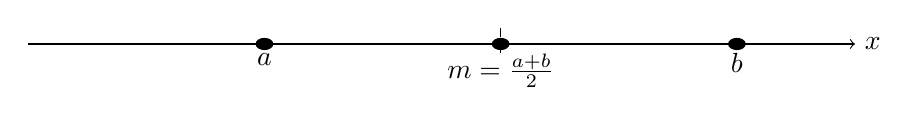
\begin{tikzpicture}[xscale=1.5, yscale=1]
  % Draw x-axis
  \draw[->] (-1,0) -- (6,0) node[right] {$x$};

  % Coordinates for a, b
  \def\a{1}
  \def\b{5}
  \def\m{3}

  % Mark points a, b, and midpoint
  \filldraw (\a,0) circle (2pt) node[below] {$a$};
  \filldraw (\b,0) circle (2pt) node[below] {$b$};
  \filldraw (\m,0) circle (2pt) node[below] {$m = \frac{a + b}{2}$};

  % Optional: Draw dashed line to show midpoint location
  \draw[dashed] (\m,0.2) -- (\m,-0.2);
\end{tikzpicture}
\end{center}

Define $f(x)$ as the quadratic function with roots $a, b$ and upward tails:
$f(x) = (x-a)(x-b)$. We know that if $x_0 = p, x_1 = q$, then a linear interpolation of 
$f$ at nodes $x_0, x_1$ on the interval $[a, b]$ satisfies: 

\begin{equation*}
    \left| f(x) - p(x) \right| = \left|\frac{ f''(\zeta_x) }{2!}\right|
    |(x-x_0)(x-x_1)| \leq
    \frac{M}{8}|x_1 - x_0|^2
\end{equation*}

with $M$ the maximum of $|f''(x)|$ in $[a, b]$ and some $\zeta_x \in (a, b)$. Now, 

\begin{equation*}
    \left| x_1 - x_0 \right|^2 = |(m+h)- (m-h)|^2 = 4h^2
\end{equation*}

Therefore, 

\begin{align*}
    &\left| \frac{ f''(\zeta_x) }{2} \right| \left| (x-p)(x-q) \right|  \leq \frac{4h^2\times M}{8}\\ 
    \Rightarrow&\left| \frac{ f''(\zeta_x) }{2} \right| \left| (x-p)(x-q) \right|  \leq
    \frac{M}{2}h^2\\
    \Rightarrow &\left| f''(\zeta_x) \right|  \left| (x-p)(x-q) \right| \leq Mh^2
\end{align*}

Here's the trick: since $f$ is quadratic, $f''$ is constant and therefore
$\left| f''(\zeta_x) \right| = |M|$. So dividing by $|M|$ on both sides we get

\begin{align*}
    \left| (x-p)(x-q) \right| \leq h^2
\end{align*}

Finally, we know $0 \leq h \leq (b-a) / 2$, so


\begin{equation*}
    \left| (x-p)(x-q) \right|  \leq h^2 \leq \left( \frac{b-a}{2} \right)^2 =
    \frac{(b-a)^2}{4}
\end{equation*}

which is what we wanted to show.

$(b)$ Let $x_0, \ldots, x_n$ s.t. $x_i = a + i\frac{(b-a)}{n}$ for $0 \leq i
\leq n$. We wish to show that for all $x \in [a, b]$,

\begin{equation*}
    \left| \eta_{n+1}(x) \right| \leq \frac{(b-a)^{n+1}}{2^{n+1}}
\end{equation*}

Take $x_i, x_{i+1}$ and let $f$ be the quadratic function with roots $x_i,
x_{i+1}$ and upward tails. Using the exact same reasoning of $(a)$, we know 

\begin{equation}
    \left| (x - x_i)(x - x_{i+1}) \right| \leq \frac{(x_{i+1} - x_{i})^2}{2^2}
\end{equation}

Since the points are equidistant, $x_{i+1} - x_{i} =  \frac{b-a}{n}$, as is easy to
prove algebraically, so equation $(2)$ is equivalent to:

\begin{equation}
    \left| (x-x_i)(x-x_{i+1}) \right| \leq \left( \frac{b-a}{2n} \right)^2
\end{equation}

See that exercise $(a)$ satisfied this formula, where had nodes $x_0, x_1$ and
therefore $n = 1$. In other words, exercise $(a)$ was the base case for an
inductive proof and we can now assume that the statement holds for $n = k - 1$
for some $k > 2$. Our inductive case consists of having points $x_0, \ldots, x_k$, where we wish to prove 

\begin{equation*}
    \left| (x - x_0)\ldots (x-x_{k-1}) \right| \leq \frac{ (b-a)^{k} }{2^{k}}
    \Rightarrow \left| (x-x_0)\ldots(x-x_{k-1})(x-x_k) \right| \leq
    \frac{(b-a)^{k+1}}{2^{k+1}}
\end{equation*}

So assume 

\begin{equation*}
    \left| \eta_{k}(x) \right| \leq \frac{(b-a)^k}{2^k}
\end{equation*}

Now take 


\begin{equation*}
    \left| \eta_{k}(x) \right| \left| (x-x_{k+1}) \right|  \leq
    \frac{(b-a)^k}{2^k} \left| (x-x_{k+1}) \right| 
\end{equation*}

Since $x \in [a, b]$ and $x_{k+1} = b$ is the last node, $\left| x - x_{k+1}
\right| \leq b-a $ (i.e. the maximum distance that $x$ can take from $b$ is when
$x$ is exactly $a$). So 

\begin{equation*}
    \left| \eta_k(x) \right| \left| (x-x_{k+1}) \right| \leq \frac{(b-a)^k}{2^k}
    \left| (x-x_{k+1}) \right|  \leq \frac{(b-a)^k}{2^k}(b-a)
\end{equation*}

Something's off. But should be along this lines.

\pagebreak 

\begin{shaded}
    \textbf{(9)} $(a)$ Let $f(x) = \cos x\pi$. Find a polynomial of degree $\leq 3$ that verifies: 

    \begin{equation*}
        p(-1) = f(-1), \qquad p(0) = f(0), \qquad p(1) = f(1), \qquad p'(1) =
        f'(1)
    \end{equation*}

    $(b)$ Find a polynomial of degree $\leq 4$ that verifies previous conditions
    and the added condition $p''(1) = f''(1)$.
\end{shaded}

$(a)$ Let $x_0 = -1, x_2 = 0, x_3 = 1$. To keep track of which nodes have double (or
more) conditions, let $z_0 = x_0, z_1 = x_1, z_2 = x_2, z_3 = x_2$ (since $x_2$
has two conditions, one for $p$ and one for $p'$.) Then, our table of divided
differences is


\begin{equation*}
    \begin{array}{c|c|c|c|c}
        z_0 & f[z_0] & f[z_0,z_1] & f[z_0,z_1,z_2]&f[z_0,z_1,z_2,z_3]  \\
z_1 & f[z_1] & f[z_1,z_2] & f[z_1,z_2,z_3]  \\
z_2 & f[z_2] & f[z_2,z_3]   \\
z_3 & f[z_3] & & & \\
\end{array}
\end{equation*}

So now we simply compute the first column.


\begin{equation*}
    \begin{array}{c|c|c|c|c}
-1 & -1 & f[z_0,z_1] & f[z_0,z_1,z_2]&f[z_0,z_1,z_2,z_3]  \\
0 & 1 & f[z_1,z_2] & f[z_1,z_2,z_3]  \\
1 & -1 & f[z_2,z_3]   \\
1 & -1 & & & \\
\end{array}
\end{equation*}

Amazing. So now we compute $f[z_2, z_3] = f[x_2, x_2]$. Since this is a repeated
node, by definition it corresponds to $f'(x_2) = f'(0)$. So, we see that 
$f'\left( 0 \right) = - \sin(0\pi) \pi = 0$. Similarly, 

\begin{equation*}
    f[z_1, z_2] = \frac{f[z_2] - f[z_1]}{z_2 - z_1} = \frac{-2}{1} = -2
\end{equation*}

and 

\begin{equation*}
    f[z_0, z_1] = \frac{f[z_1] - f[z_0]}{z_1 - z_0} = 2
\end{equation*}

So,

\begin{equation*}
    \begin{array}{c|c|c|c|c}
-1 & -1 & 2 & f[z_0,z_1,z_2]&f[z_0,z_1,z_2,z_3]  \\
0 & 1 & -2 & f[z_1,z_2,z_3]  \\
1 & -1 & 0   \\
1 & -1 & & & \\
\end{array}
\end{equation*}

Now, 

\begin{equation*}
    f[z_1, z_2, z_3] = \frac{ f[z_2, z_3] - f[z_1, z_2] }{z_3 - z_1} =
    \frac{2}{1} = 2
\end{equation*}

\begin{equation*}
    f[z_0, z_1, z_2] = \frac{ f[z_1, z_2] - f[z_0, z_1] }{z_2 - z_0} =
    -\frac{2}{2} = -2
\end{equation*}

\begin{equation*}
    \begin{array}{c|c|c|c|c}
-1 & -1 & 2 & -2&f[z_0,z_1,z_2,z_3]  \\
0 & 1 & -2 & 2  \\
1 & -1 & 0   \\
1 & -1 & & & \\
\end{array}
\end{equation*}

At last, 

\begin{equation*}
    f[z_0, \ldots, z_3] = \frac{f[z_1, z_2, z_3] - f[z_0, z_1, z_2]}{z_3 - z_0}
    = 2
\end{equation*}

The interpolating polynomial is built using Newton's form---remember that
$f[x_0], f[x_0,x_1], \ldots$ etc are the coefficients $c_0, c_1, \ldots$ in
Newton's form $\sum_{i=0}^n c_i \eta_i(x)$. So,

\begin{equation*}
    p(x) = f[z_0] + f[z_0, z_1](x-z_0) + f[z_{0}, z_1, z_2](x-z_0)(x-z_1) +
    f[z_0,\ldots, z_3](x-z_0)(x-z_1)(x-z_2)
\end{equation*}

Simplifying,

\begin{align*}
    p(x) 
    &= -1 +2(x+1) -2 (x+1)x + 2(x+1)x(x-1)
\end{align*}

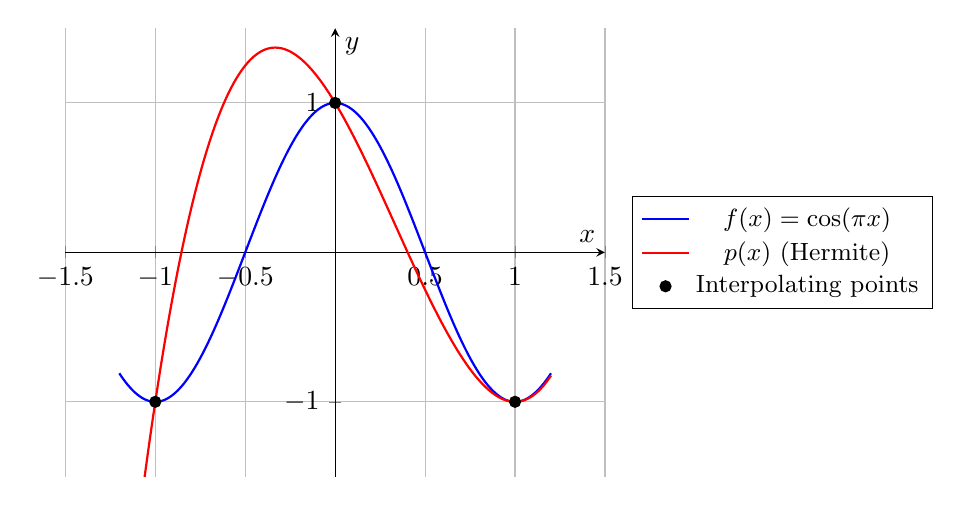
\begin{tikzpicture}
\begin{axis}[
    axis lines=middle,
    xlabel={$x$},
    ylabel={$y$},
    xmin=-1.5, xmax=1.5,
    ymin=-1.5, ymax=1.5,
    grid=both,
    samples=200,
    legend style={
        at={(1.05,0.5)},
        anchor=west,
        font=\small
    }
]

% Plot f(x) = cos(pi x)
\addplot[blue, thick, domain=-1.2:1.2] {cos(deg(pi*x))};
\addlegendentry{$f(x) = \cos(\pi x)$}

% Plot p(x)
\addplot[red, thick, domain=-1.2:1.2] {-1 +2*(x+1) -2*(x+1)*x + 2*(x+1)*x*(x-1)};
\addlegendentry{$p(x)$ (Hermite)}

% Add interpolation points
\addplot[only marks, mark=*, black] coordinates {
    (-1, -1)
    (0, 1)
    (1, -1)
};
\addlegendentry{Interpolating points}

\end{axis}
\end{tikzpicture}

\pagebreak 

\begin{shaded}
    \textbf{(10)} We wish to approximate $f(x) = \sqrt{x} $ with an error of at
    most $5 \times 10^{-8}$ using a linear spline and quadratic interpolation
    every three nodes. 

    Determine the least number of nodes $n$ of the form $x_i = 1 + \frac{i}{n}$,
    with $i = 0, \ldots, n$, and interval length $h$, so that the error bound is
    met.
\end{shaded}

(Linear spline) See that the desired approximation falls within $[1, 2]$. For a
linear spline, the error of approximation obeys 

\begin{equation*}
    \left| e(x) \right| < \frac{M}{8}h^2, \qquad x \in [1, 2] \text{ and } M =
    \max |f''|
\end{equation*}

where we can think of $h$ as a function of $n$, i.e. $h(n) = \frac{1}{n}$ for
$n \in \mathbb{N}$. 

\begin{align*}
    &\frac{M}{8}h(n)^2 \leq 5 \times 10^{-8} \\ 
    \iff&\frac{M}{( n )^2} \leq 40 \times 10^{-8} \\ 
    \iff& \frac{10^8M}{40} \leq n^2 \\ 
    \iff&\sqrt{\frac{10^8 M}{40}} \leq n 
\end{align*}

Now, suffices to see that 

\begin{equation*}
    f'(x) = \frac{1}{2\sqrt{x} }, \qquad f''(x) = -\frac{1}{4 x^{3 / 2}}
\end{equation*}

Clearly then $|f''(x)|$ is decreasing and its maximum in $[1, 2]$ occurs at $x =
1$ :

\begin{equation*}
M = |f''(1))| = \frac{1}{4}
\end{equation*}

So, we require 

\begin{align*}
    &\sqrt{\frac{10^8}{40 \times 4}}   \leq n \\ 
    \iff& \frac{10^4}{\sqrt{160} }  \leq n \\ 
    \iff& \frac{10.000}{\sqrt{16 \times 10} }  \leq n \\
    \iff& \frac{10.000}{4\sqrt{10} }  \leq n \\
    \iff& \frac{2500}{\sqrt{10} }  \leq n \\
    \iff&790.569 \leq n
\end{align*}

So fixing $n = 791$ suffices.

(Quadratic interpolation) Assume we group $x_0, \ldots, x_n$ into $x_0,x_1,x_2$,
then $x_3,x_4,x_5$, etc. Let $\overrightarrow{x}_i$ denote the $i$th grouping of
three nodes. We are of course assuming that there are $n+1 = 3k$ nodes with $k
\in \mathbb{N}$. The function $h(n)$ which specifies the distance between nodes
will be specified later.

Assume each $\overrightarrow{x}_i$ is used to fit a quadratic polynomial $q_i(x)
= a_ix^2 + b_ix + c_i$. The error of interpolation will then be specific to each
interval. In other words, for any $x$ belonging to the interval specified by
$\overrightarrow{x}_i$, 

\begin{equation*}
    \left| e(x) \right| = \left|\frac{ f^{(3)}(\zeta_x) }{3!}\prod_{\widetilde{ x }
    \in \overrightarrow{x}_i } (x-\widetilde{ x } )\right|
\end{equation*}

for some $\zeta_x$ in the interval of interest. Taking $M = \max \left| f^{(3)}
(x)\right| $, with $f^{(3)}(x) = \frac{3}{8x^{\frac{5}{}}}$, we obtain $M
= 3 / 8$. Now the question becomes whether we can bound the factorial
expression. See that 

\begin{equation*}
    \varphi(x) = (x-x_0)(x-x_1)(x-x_2)
\end{equation*}

is a cubic function with distinct roots. (We could have chosen any successive
values for $x_0,x_1,x_2$.) Consider $\varphi$ as restricted to the interval
$[x_0, x_2]$. We know that it will have three roots, a maximum $x_M$ in $[x_0, x_1]$
and a minimum $x_m$ at $[x_1, x_2]$. Since the roots are equidistant (root
symmetry), $\varphi$ is symmetric around the mid-root $x_1$ and $\varphi(x_m) =
\varphi(x_M)$. But where is the critical point? 

\begin{shaded}
    $(\star)$ Let us consider a centered cubic polynomial, without loss of
    generality. Let $\phi(x) = (x-a)x(x-b)$, with mid-root zero. Assuming root
    symmetry, $a = -b$. So letting $r = b$ we have 

    \begin{equation*}
        \phi(x) = (x-r)x(x+r) = x^3 -xr^2
    \end{equation*}

    Its derivative $\phi'(x) = 3x^2 - r^2$ is zero if and only if $x = \pm
    \frac{r}{\sqrt{3} }$. We have already established that these critical points
    are equal in their absolute values. Now it only suffices to see that 

    \begin{equation*}
        \phi\left( \frac{r}{\sqrt{3} } \right)  = - \frac{2r^3}{3\sqrt{3} } =-
        \frac{(c-a)^3}{12\sqrt{3} }
    \end{equation*}

    (because $r = (c-a) / 2$). Therefore,

    \begin{equation*}
        \max |\phi(x)| = \frac{(c-a)^3}{12 \sqrt{3} }
    \end{equation*}


\end{shaded}

From $( \star )$ readily follows that 

\begin{equation*}
    \left| \prod_{\widetilde{ x } \in \overrightarrow{x}_i }(x-\widetilde{ x } )
    \right| \leq \frac{ h^3 }{12\sqrt{3} }
\end{equation*}

where $h$ is the distance between the last node in a grouping and the first
(i.e. $x_2 - x_0 = x_5 - x_3 = \ldots$ etc.) In consequence, 


\begin{align*}
    \left| e(x) \right| = \left|\frac{ f^{(3)}(\zeta_x) }{3!}\prod_{\widetilde{ x }
    \in \overrightarrow{x}_i } (x-\widetilde{ x } )\right| \\ 
    \Rightarrow \left| e(x) \right| \leq  3 / 8 \frac{h^3}{12\sqrt{3} }
\end{align*}

Here, $h$ is a function of $n$. If $n = 2$ (three points), then $h = 2/3$.
If $n = 5$ (six points), then each sub-interval is of length $1 / 6$ and $h =
2/6$. In general, if $n = 3k$, then $h = \frac{2}{n}$. So we have 

\begin{equation*}
    \left| e(x) \right|  \leq \frac{ 3 }{8\times \sqrt{3} } \frac{2}{n} =
    \frac{3}{4\sqrt{3}n }
\end{equation*}

So now all that is needed is to bound the RHS expression to $5 \times 10^{-8}$:

\begin{equation*}
    \frac{3}{4\sqrt{3}n } \leq 5\times 10^{-8} \iff \ldots
\end{equation*}

bla bla. This is the simplest part of the problem so I skip it.

\pagebreak 

\begin{shaded}
    \textbf{(10)} Let $f(x) = \cos x$. Determine the step-length $h$ and minimum
    number of nodes $n+1$ needed to approximate $f(x)$ via linear spline in $[0,
    2\pi]$ with an error less than or equal to $5 \times 10^{-7}$.
\end{shaded}

We know 

\begin{equation*}
    \left| e(x) \right| \leq \frac{M}{8}h(n)^2
\end{equation*}

where $h(n) = \frac{2\pi}{n}$ anda $M = \max \left| f''(x) \right| $. Since
$f''(x) = -\cos x$, its maximum in $[0, 2\pi]$ is $1$. From this follows that 

\begin{equation*}
    \left| e(x) \right|  \leq \frac{4\pi^2}{8n^2} = \frac{1}{2}\left(
    \frac{\pi}{n} \right)^2
\end{equation*}

and all that is left is bounding said expression to be less than or equal to $5
\times 10^{-7}$. If one does the math, we obtain that said condition holds iff 
$n = \geq \pi \times 10^3 \approx 3141.59$, which means letting $n = 3142$
suffices. So the number of nodes needed is $n+1 = 3143$. The step length 
$h$ results $\frac{2\pi}{3142} \approx 0.001999 \approx 0.002$.

\pagebreak 

\begin{shaded}
    \textbf{(12)} $(a)$ Determine $\alpha, \beta, \gamma$ such that 

    \begin{equation*}
        S(x) = \begin{cases}
            \alpha x^3 + \gamma x & 0 \leq x \leq 1 \\ 
            -\alpha x^3 + \beta x^2 - 5\alpha x + 1 & 1 \leq x \leq 2
        \end{cases}
    \end{equation*}

    is a cubic spline.

    $(b)$ With the determined values, decide if $S$ interpolates $f(x) = 2^x +
    1 / 2 x^2 - 1 / 2 x - 1$ in $[0, 2]$  with nodes $\left\{ 0, 1, 2 \right\}
    $. 

    $(c)$ Graph $f$ and $S$ in $[0, 2]$.
\end{shaded}

$(a)$ $S(x)$ must satisfy the interpolation constraint and the continuity
constraint. Note that $S(x)$ are polynomials with continuous first and second
derivatives in $[0, 2]$. Furthermore, 

\begin{equation*}
    S'(x) = \begin{cases}
        3\alpha x^2 + \gamma & 0 \leq x \leq 1 \\ 
        -3\alpha x^2 + 2\beta x - 5\alpha & 1 \leq x \leq 2
    \end{cases}, \qquad S''(x) = \begin{cases}
        6\alpha x & 0 \leq x \leq 1 \\ 
        -6\alpha x + 2 \beta & 1 \leq x \leq 2
    \end{cases}
\end{equation*}

For all $f$ in $\left\{ S, S', S'' \right\} $ we wish that

\begin{equation*}
    \lim_{x \to 1 (\leftarrow)} f(x) = \lim_{x \to 1(\rightarrow)} f(x)
\end{equation*}

$(a.a)$ Beginning with $S''(x)$, we impose

\begin{equation*}
    6\alpha = -6\alpha + 2\beta \Rightarrow 12\alpha = 2 \beta \Rightarrow \beta
    = 6\alpha
\end{equation*}

$(a.b)$ Now taking $S'(x)$, we impose 

\begin{equation*}
    3\alpha + \gamma = -3\alpha + 2\beta -5\alpha
\end{equation*}

Substituting with $\beta = 6\alpha$, we find 

\begin{equation*}
    \gamma = -6\alph\alpha + 2(6\alpha) -5\alpha \Rightarrow \gamma = \alpha
\end{equation*}

$(a.c)$ Now taking $S(x)$, we impose 

\begin{equation*}
    \alpha + \gamma = -\alpha + \beta - 5\alpha + 1
\end{equation*}

Substituting with $\gamma = \alpha, \beta = 6\alpha$, we find 

\begin{equation*}
    2\alpha = 1 \Rightarrow \alpha = \frac{1}{2}
\end{equation*}

So we finally obtain 

\begin{equation*}
    \alpha = \frac{1}{2}, \beta = 3, \gamma = \frac{1}{2}
\end{equation*}

$(b)$ It is simple to see that the spline does interpolate $f$ simply by
evaluating $S$ and $f$ on $0, 1, 2$.

$(c)$

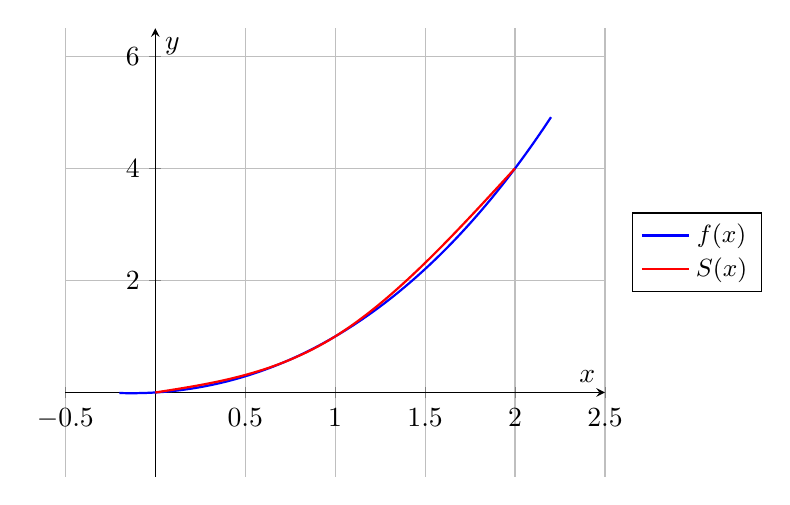
\begin{tikzpicture}
\begin{axis}[
    axis lines=middle,
    xlabel={$x$},
    ylabel={$y$},
    xmin=-0.5, xmax=2.5,
    ymin=-1.5, ymax=6.5,
    grid=both,
    samples=200,
    legend style={
        at={(1.05,0.5)},
        anchor=west,
        font=\small
    }
]

% Plot f(x) = cos(pi x)
\addplot[blue, thick, domain=-0.2:2.2] {2^x + 1/2 * x^2 - 1/2 * x - 1};
\addlegendentry{$f(x)$}

% Plot p(x)
\addplot[red, thick, domain=0:1] {1/2 * x^3 + 1/2 * x};
\addplot[red, thick, domain=1:2] {-1/2 * x^3 + 3 * x^2 - 5*(1/2)*x + 1};
\addlegendentry{$S(x)$}

\end{axis}
\end{tikzpicture}


\section{Function approximation}

\subsection{Least squares method}

Assume $(x_1, y_1), \ldots (x_m, y_m)$ are points from a function $f$ we wish to
approximate. A reasonable approach is to find a linear function with
coefficients $a_0, a_1$ that minimize

\begin{equation*}
    E = \sum_{i=1}^m \left( y_i - (a_1 x_i + a_0) \right)^2
\end{equation*}

Doing the standard things (take partial derivative, equate it to zero, etc.) we
obtain the following normal equations to minimize $E$:

\begin{equation*}
    a_0 = \frac{\left( \sum x_i^2 \right)\left( \sum y_i \right) - \left( \sum
    x_i y_i \right) \left( \sum x_i \right)    }{m\sum x_i^2 - \sum x_i}, \qquad
    a_1 = \frac{m \sum x_i y_i - \left( \sum x_i \right)\left( \sum y_i \right)  }
    {m \sum x_i^2 - \sum x_i}
\end{equation*}

where all sums range from $i = 1$ to $m$. 

The general case is when $f$ is approximated with a polynomial of degree $\leq
n$, with $n < m - 1$. Now, we need to determine the coefficients $a_0, \ldots,
a_n$ that minimize 

\begin{equation*}
    \sum_{i=1}^m \left( y_i - p_n(x_i) \right)^2
\end{equation*}

Again, doing the standard procedure, the following system of equation emerges
for variables $a_0, \ldots, a_n$: 

\begin{equation*}
    \begin{bmatrix} 
        \sum x_i^0 & \sum x_i^1 & \sum x_i^2  & \ldots & \sum x_i^n  \\ 
        \sum x_i^1 & \sum x_i^2 & \sum x_i^3 & \ldots & \sum x_i^{n+1} \\ 
        \vdots & \vdots & \vdots & \ldots & \vdots \\ 
        \sum x_i^2 & \sum x_i^{n+1} & \sum x_i^{n+2} & \ldots & \sum x_i^{2n}
    \end{bmatrix} \begin{bmatrix} 
            a_0 \\ a_1 \\ \vdots \\ a_n 
    \end{bmatrix} = \begin{bmatrix} 
            \sum y_ix_i^0 \\ 
            \sum y_ix_i^1 \\ 
            \vdots \\ 
            \sum y_i x_i^n
    \end{bmatrix} 
\end{equation*}

\subsection{Non-polynomial models}

It is possible to propose a non-polynomial model for $f$, e.g. $\hat{f}(x) = b
e^{ax}$ or whatever. This produces a non-linear system of equations which cannot
be solved simply. However, taking the logarithm of the proposed model allows for
a linear approximation. For example, if $\hat{f}(x) = be^{ax}$ then 

\begin{equation*}
    \ln \hat{f}(x) = \ln b + ax
\end{equation*}

which is a linear model that can be fitted using least squares. However, it is
important to recall that the values $y_1, \ldots, y_m$ must be scaled with $\ln
y_1, \ldots, \ln y_m$ to fit the logarithmic model.

\subsection{Error of approximation}

Assume $f \in C[a, b]$ and $P_n(x)$ of degree $\leq n$ an approximation via
least squares. Then 

\begin{equation*}
    E = E(a_0, \ldots, a_n) = \int_a^b \left( f(x) - P_n(x) \right)^2 ~ dx =
    \int_a^b \left[ f(x) \ sum_{k=0}^n a_k x^k \right]^2 ~ dx
\end{equation*}

In general, we wish to find $a_0, \ldots, a_n$ such that $E$ is minimal. In
general, the partial derivative of $E$ with respect to $a_j$ is zero 
if and only if 

\begin{equation*}
    \sum_{k=0}^n \left( a_k \int_a^b x^{k+j} ~ dx \right)  = \int_a^b x^j f(x) ~ dx, \qquad j =
    0, \ldots, n
\end{equation*}

This readily provides a $(n+1) \times (n+1)$ system of equations which is to be solved to minimize
the error:

\begin{equation*}
    \begin{bmatrix} 
        \int_a^b ~ dx & \int_a^b x ~ dx & \ldots & \int_a^b x^{n} \\ 
        \int_a^b x ~ dx & \int_a^b x^2 ~ dx & \ldots & \int_a^b x^{n+1} \\ 
        \vdots & \vdots & \ldots & \vdots \\ 
        \int_a^b x^n & \int_a^b x^{n+1} & \ldots & \int_a^b x^{2n}
    \end{bmatrix} \begin{bmatrix} 
            a_0 \\ a_1 \\ \vdots \\ a_n 
    \end{bmatrix} = \begin{bmatrix} 
            \int_a^b x^0 f(x) ~ dx \\  
            \int_a^b x f(x) ~ dx \\ 
            \vdots \\ 
            \int_a^b x^n f(x) ~ dx
    \end{bmatrix} 
\end{equation*}

Notice that, in LHS matrix, the coefficient $c_{jk}$ is 

\begin{equation*}
    \int_a^b x^{j+k} ~ dx = \frac{b^{j+k+1} - a^{j+k+1}}{j+k+1}
\end{equation*}

which allows for a more direct computation of the system. The LHS matrix is
called \textbf{Hilbert matrix} and it is famously ill-conditioned---i.e. small
changes in the coefficients greatly affect the final result. 

\subsection{A few polynomial theorems}

Recall that vectors $\phi_1, \ldots, \phi_n$ are linearly independent if
$\sum_{i=0}^n c_i \phi_i = 0$ entails that $c_0 = \ldots = c_n = 0$. In
particular, a function space $\mathcal{F}$ is a vector space 
such that $\Pi = \bigcup_{i=0}^\infty \Pi_i \subseteq \mathcal{F}$. 

\begin{theorem}[Polynomials of different degrees are linearly independent]
    Let $\phi_0, \ldots, \phi_n$ such that $\phi_j \in \Pi_j$. Then $\left\{ \phi_i
    \right\}_{i=0}^n $ is linearly independent in any interval 
    $[a, b]$.
\end{theorem}


\small
\begin{quote}

\textbf{Proof.} Assume $c_0, \ldots, c_n$ are such that $P(x) = c_0\phi_0(x) + \ldots +
c_n \phi_n(x) = 0$ for any $x \in [a, b]$.  Since $P(x)$ is null 
for all $x$ in $[a, b]$, each exponentiation $x^k$ must be zero. 
Since $c_n \phi_n(x)$ is the only term which includes $x^n$,
we must have $c_n = 0$, which readily entails $P(x) = c_0 \phi_0(x) + \ldots +
c_{n-1}\phi_{n-1}(x)$. By recurrence, $c_0 = \ldots = c_n = 0$. $\blacksquare$

\end{quote}
\normalsize

The previous theorem is highly general, since any polynomial of degree $n$ is by
definition a linear combination of $n+1$ polynomials of degree $0, 1, \ldots, n$.
For instance, $1 + 3x + 2x^2$ can be considered a linear combination of the
polynomials $1, x, x^2$ with coefficients $1, 3, 2$, or of the polynomials 
$1, 3x, 4x^2$ with coefficients $1, 1, 1 / 2$, etc.

\begin{theorem}
    Let $\left\{ \phi_0, \ldots, \phi_n \right\} $ be a set of linearly
    independent polynomials for any interval $[a, b]$, each of degree 
    $\leq n$. Then any polynomial of degree $\leq n$ can be expressed as a
    linear combination of $\left\{ \phi_0, \ldots, \phi_n \right\} $.
\end{theorem}

\subsection{Weighted function approximation: Diagonalizing Hilbert matrix}

A weight function $\omega(x)$ on interval $I$ is a function such that:

\begin{enumerate}
    \item $\omega(x) > 0$ for all $x \in I$. 
    \item $\omega(x) \neq 0$ for all $x$ in any arbitrary sub-interval of $I$.
\end{enumerate}

Condition $(2)$ means that $\omega$ cannot be constantly zero in any
sub-interval, i.e. any zero mapping of $\omega$ must be a point.
Weight function allow one to give more or less importance to approximations 
in different regions of an interval of interest. 

Now assume we have a linearly independent set of functions $\left\{ \phi_0,
\ldots, \phi_n \right\} $ in $[a, b]$, a weight function $\omega$ defined on
$[a, b]$, and $f$ continuous in $[a, b]$ which we wish to approximate. Then 
there is a set of coefficients $a_0, \ldots, a_n$ of 

\begin{equation*}
    P(x) = \sum_{k=0}^n a_k \phi_k(x)
\end{equation*}

that minimize the following error function:

\begin{equation*}
    E = E(a_0, \ldots, a_n) = \int_a^b \omega(x)\left[ f(x) -P(x) \right]^2 ~ dx
\end{equation*}

This is the same as we did before: we are approximating $f$ via a polynomial by
finding the coefficients that minimize the error of approximation. But now we
are $(a)$ including a weight function and $(b)$ defining $P(x)$ as a linear
combination of independent polynomials. 

Once more, taking the derivative of $E$ with respect to an arbitrary $a_j$, we
find that said derivative is zero if and only if 

\begin{equation*}
    \sum_{k=0}^n a_k \int_a^b \omega(x)\phi_k(x) \phi_j(x) ~ dx = \int_a^b
    \omega(x) f(x)0 \phi_j(x) ~ dx, \qquad j = 0, \ldots, n
\end{equation*}

which readily provides a system of equations. The system is complex, but it can
be greatly simplified if we could choose $\left\{ \phi_0, \ldots, \phi_n \right\} $
such that 

\begin{equation*}
    \int_a^b \omega(x) \phi_k(x) \phi_j(x) ~ dx = \alpha_j \delta_{jk}
\end{equation*}

for some $\alpha_j > 0$. In that case, the equation would simplify to 

\begin{equation*}
    a_j \int_a^b \omega(x) \phi_j^2(x) ~ dx = \int_a^b \omega(x) f(x) \phi_j(x)
    ~ dx, \qquad j = 0, \ldots, n
\end{equation*}

By assumption, this would yield

\begin{equation*}
    a_j \alpha_j = \int_a^b \omega(x) f(x) \phi_j(x)~ dx, \qquad j = 0, \ldots,
    n
\end{equation*}

or equivalently 

\begin{equation*}
    a_j = \frac{1}{\alpha_j} \int_a^b \omega(x) f(x) \phi_j(x) ~ dx, \qquad j =
    0, \ldots, n
\end{equation*}

In short, a relatively simple system of equations emerges if $\phi_0, \ldots,
\phi_n$ are intelligently chosen. But how to choose them intelligently? 

\begin{definition}[Ortogonal set]
    A set $\left\{ \phi_0, \ldots, \phi_n \right\} $ of functoins defined in
    $[a, b]$ is ortogonal with respect to a weight function $\omega$ iff 

    \begin{equation*}
        \int_a^b \omega(x) \phi_k(x) \phi_j(x) ~ dx = \alpha_j \delta_{jk},
        \qquad j = 0, \ldots, n
    \end{equation*}

    for $\alpha_j > 0$. If $\alpha_j = 1$ for all $j = 0, \ldots, n$ then we say
    the set is ortonormal.
\end{definition}

We can formalize what was said so far as follows:

\begin{theorem}[Ortogonal polynomial approximation theorem]
    If $\left\{ \phi_0, \ldots, \phi_k \right\} $ defined in $[a, b]$ is
    ortogonal with respect to $\omega$ defined in $[a, b]$,
    then the least squared approximation of $f$ weighted by $\omega$ is 

    \begin{equation*}
        P(x) = \sum_{k=0}^n a_k \phi_k(x)
    \end{equation*}

    with 

    \begin{equation*}
        a_k = \frac{1}{\alpha_k} \int_a^b \omega(x) f(x) \phi_k(x) ~ dx
    \end{equation*}

    where $\alpha_k = \int_a^b \omega(x) \phi_k^2(x) ~ dx$.
\end{theorem}

\begin{theorem}[Ortogonal set generation]
    The following is an ortogonal set of functions defined in $[a, b]$ with 
    respect to a weight function $\omega$: 

    \begin{equation*}
        \phi_0(x) = 1, \qquad \phi_1(x) = x-B_1, \qquad x \in [a, b]
    \end{equation*}

    where 

    \begin{equation*}
        B_1 = \frac{\int_a^b x \omega(x) \phi_0^2(x) ~ dx}{\int_a^b \omega(x)
        \phi_0^2(x) ~ dx}
    \end{equation*}

    For $k \geq 2$, 

    \begin{equation*}
        \phi_k(x) = (x - B_k) \phi_{k-1}(x) - C_k \phi_{k-2}(x), \qquad x \in
        [a, b]
    \end{equation*}

    with 

    \begin{equation*}
        B_k = \frac{\int_a^b x \omega(x) \phi^2_{k-1}(x) ~ dx}{\int_a^b
        \omega(x) \phi^2_{k-1}(x)}, \qquad C_k = \frac{\int_a^b x \omega(x)
    \phi_{k-1}(x) \phi_{k-2}(x) ~ dx}{\int_a^b \omega(x) \phi^2_{k-2}(x) ~ dx}
    \end{equation*}
\end{theorem}

In general, we will use a few ortogonal sets which are already known, built
recurrently from the previous theorem: 

\begin{enumerate}
    \item \textbf{Legendre polynomials}:

        \begin{equation*}
            \phi_0(x) = 1, \phi_1(x) = x, \phi_2(x) = x^2 - \frac{1}{3},
            \phi_3(x) = x^3 - \frac{3}{5}x, \phi_4(x) = x^4 - \frac{6}{7}x^2 +
            \frac{3}{25}, \ldots
        \end{equation*}

    \item More examples in the textbook.

\end{enumerate}

\pagebreak 

\subsection{Exercises}

\begin{shaded}
    \textbf{(1)} Approximate $f(x)$ with a polynomial of degree $1$ and $g(x)$ with a
    polynomial of degree two, where: 

     \begin{equation*}
    \begin{array}{c|c|c|c|c|c|c|c|c|c|c}
        x & 0 & 1 & 2 & 3 & 4 & 5 & 6 & 7 & 8 & 9\\
        \hat{f}(x) & -0.1 & 1.1 & 1.9 & 3.2 & 3.8 & 5.0 & 6.0 & 7.3 & 8.1 & 8.9
     \end{array}
     \end{equation*}

     and 

     \begin{equation*}
    \begin{array}{c|c|c|c|c|c}
        x & -1 & 0 & 1 & 3 & 6\\ 
        \hat{g}(x) & 6.1 & 2.8 & 2.2 & 6 & 26.9
     \end{array}
     \end{equation*}

\end{shaded}

$(f)$ We know $p(x) = a_0 + a_1x + \ldots + a_nx^n$ is the least squared
approximation of $f$ if and only if $a_0, \ldots, a_n$ are solutions to the
following system of equations: 

\begin{equation*}
    \begin{bmatrix} 
        \sum_{i=0}^m x_i^0 & \sum_{i=0}^m x_i^1 & \ldots & \sum_{i=0}^m x_i^m
        \mid \sum_{i=0}^m x_i^0 y_i\\ 
        \sum_{i=0}^m x_i^1 & \sum_{i=0}^m x_i^2 & \ldots & \sum_{i=0}^{m+1} x_i^m
        \mid \sum_{i=0}^m x_i^1 y_i\\ 
        \vdots & \vdots & \ldots & \vdots & \\

        \sum_{i=0}^m x_i^m & \sum_{i=0}^m x_i^{m+1} & \ldots & \sum_{i=0}^m
        x_i^{2m}
        \mid \sum_{i=0}^m x_i^m y_i\\ 
    \end{bmatrix} 
\end{equation*}

where $m$ is the number of points $(x_i, \hat{f}(x_i))$. Since we wish to
approximate $f$ with a polynomial of degree $1$, this gives a $2\times 2$ matrix 
with coefficients

\begin{align*}
    &c_{11} = \sum_{i=0}^9 (1) = 10, \qquad c_{11} = \sum_{i=0}^9 x = 45, \\
    &c_{21} = \sum_{i=0}^9 x_i = 45, \qquad c_{22} = \sum_{i=0}^n x_i^2 = 285 
\end{align*}

The solution vector, on the other hand, is: 

\begin{equation*}
    w_{1} = \sum_{i=0}^9 y_i = 45.2, \qquad w_2 = \sum_{i=0}^9 x_i y_i = 286.7
\end{equation*}

So, suffices to solve the system 

\begin{equation*}
    \begin{bmatrix} 
    10 & 45 & 45.2 \\ 
    45 & 285 & 286.7
    \end{bmatrix} \to \begin{bmatrix} 
    1 & 4.5 & 4.52 \\ 
    1 & 6.33 & 6.371 
    \end{bmatrix} \to \begin{bmatrix} 
    1 & 4.5 & 4.52\\
    0 & 1.83 & 1.85 
    \end{bmatrix} 
\end{equation*}

So $a_1 = \frac{1.85}{1.83} a_2 = 1.01 a_2$, bla bla. Linear system, cursillo de
ingreso.

$(g)$ Not that different from $(f)$: calculate the matrix, which will be
$3\times 3$ now (degree two polynomial), solve the resulting system.
Calculating the matrix is computing sums (stupid), solving the system is solving
a linear system (stupid).

\pagebreak 

\begin{shaded}
    \textbf{(2)} Prove  that with $n + 1$ distinct points, the best polynomial
    approximation (in the sense of least squares) of degree $n$ coincides with
    the interpolating polynomial.
\end{shaded}

Let $p_n(x)$ be the interpolating polynomial of $f$ on points $x_0, \ldots,
x_n$. Let $\ell_n(x)$ be the least squares approximation of degree $n$.
Observe that 

\begin{equation*}
    \sum_{i=0}^n (y_i - p_n(x_i))^2 = 0
\end{equation*}

Since $\ell_n(x)$ minimizes the error among all polynomials of degree $n$,
and taking $p_n$ we have an error of zero, we must have 

\begin{equation*}
    \sum_{i=0}^n (y_i - \ell_n(x))^2 = 0 
\end{equation*}

which holds if and only if $\ell_n(x)$ is an interpolating polynomial. But the
interpolating polynomial is unique. $\therefore ~ p_n(x) = \ell_n(x)$.


\pagebreak 

\begin{shaded}
    \textbf{(3)} Find the polynomial of degree $0$ that best approximates 
    $f : [a, b] \to \mathbb{R}$ on $x_1, \ldots, x_n$ in $[a, b]$.
\end{shaded}

We wish to find a constant polynomial $p_0(x) = c$ such that 

\begin{equation*}
    S = \sum_{i=1}^n \left[ y_i - p_0(x_i) \right]^2 = \sum_{i=1}^n \left[ y_i - c
    \right]^2
\end{equation*}

is minimized. Taking 

\begin{align*}
    \frac{\partial S}{\partial c} 
    &= \sum_{i=1}^n \frac{\partial }{\partial c}
    (y_i - c)^2\\ 
    &=\sum_{i=1}^n \frac{\partial u^2}{\partial u} \frac{\partial }{\partial
    c}(y_i - c) \\ 
    &= \sum_{i=1}^n 2(y_i - c)(-1) \\ 
    &=2 \sum_{i=1}^n (c - y_i) \\ 
    &=2 \left( cn - \sum_{i=1}^n y_i \right) 
\end{align*}

The expression above is zero if and only if 

\begin{equation*}
    c = \frac{1}{n} \sum_{i=1}^n y_i
\end{equation*}

Therefore, the constant polynomial which best approximates $f$ (in the sense of
least squares) is the one whose value is the mean of $y_1, \ldots, y_n$.

\pagebreak 

\begin{shaded}
    \textbf{(4)} Approximate the following data with a model of the form $f(x) \sim ae^{bx}$. 


     \begin{equation*}
    \begin{array}{c|c|c|c|c}
        x & -1 & 0 & 1 & 2\\ 
        y & 8.1 & 3 & 1.1 & 0.5 
     \end{array}
     \end{equation*}
\end{shaded}

If $f(x) = ae^{bx}$ then $g(x) = \ln \left( f(x) \right) = \ln a + bx$.
Now take the logarithm of the sampled image of $f$:


     \begin{equation*}
    \begin{array}{c|c|c|c|c}
        x & -1 & 0 & 1 & 2\\ 
        y & 2.09 & 1.09 & 0.09 & -0.69 
     \end{array}
     \end{equation*}

We can fit the linear model $g(x) = \ln a + bx$ to this data using the standard
procedure. The $2\times 2$ matrix associated to the system whose solutions are
$\ln a, b$ is given by: 

\begin{align*}
    &\sum_{i=0}^3 x^0 = 4, \qquad \sum_{i=0}^3 x_i 2, \qquad \sum_{i=0}^3 x_i^2
    = 6, \\ 
    &\sum_{i=0}^3 x_i^0 y_i = 2.58, \qquad \sum_{i=0}^3 x_i y_i = -3.38
\end{align*}

In other words, the system is 

\begin{equation*}
    \begin{bmatrix} 
        4 & 2 &2.58 \\ 
        2 & 6  & -3.38
        \end{bmatrix} \Rightarrow \begin{bmatrix} 
        1 & 0 & 1.112 \\ 
        0 & 1 & -0.934
    \end{bmatrix}   
\end{equation*}

From this follows: 

\begin{equation*}
    \ln a = 1.112 ~ (\text{or } a = e^{1.112} \approx 3.04), \qquad b = -0.934
\end{equation*}

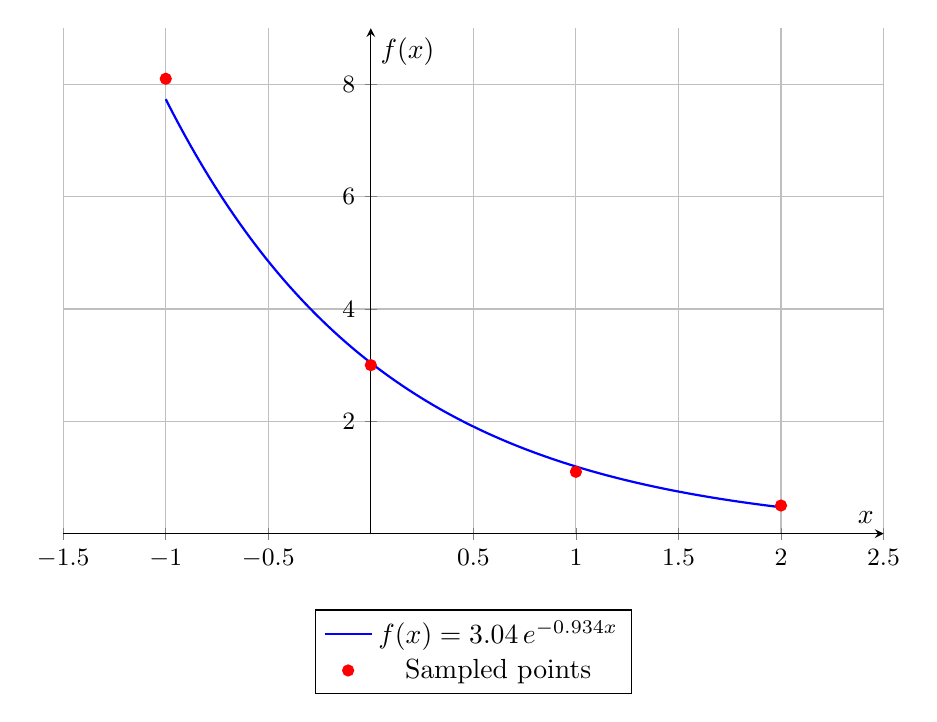
\begin{tikzpicture}
  \begin{axis}[
    width=12cm,
    height=8cm,
    axis lines=middle,
    xlabel={$x$},
    ylabel={$f(x)$},
    xmin=-1.5, xmax=2.5,
    ymin=0, ymax=9,
    domain=-1:2,
    samples=100,
    grid=both,
    legend style={at={(0.5,-0.15)},anchor=north},
    ticklabel style={font=\small}
  ]

    % Plot the exponential function
    \addplot[
      thick,
      blue
    ] {3.04*exp(-0.934*x)};
    \addlegendentry{$f(x) = 3.04\, e^{-0.934x}$}

    % Plot the given data points
    \addplot[
      only marks,
      mark=*,
      red,
      mark size=2pt
    ] coordinates {
      (-1, 8.1)
      (0, 3)
      (1, 1.1)
      (2, 0.5)
    };
    \addlegendentry{Sampled points}

  \end{axis}
\end{tikzpicture}

\pagebreak 

\begin{shaded}
    \textbf{(5)} Same, but with $f(x) \sim -e^{ax^2 + bx + c}$ and values


     \begin{equation*}
    \begin{array}{c|c|c|c|c}
        x & -1 & 0 & 1 & 2\\ 
        y & -1.1 & -0.4 & -0.9 & -0.5
     \end{array}
     \end{equation*}
\end{shaded}

An obvious problem is that $\mathcal{D}(\ln) = \mathbb{R}^+$. So take 

\begin{equation*}
    \phi(x) = \ln\left( - f(x) \right) = ax^2 + bx + c
\end{equation*}

so that the transformation we need to apply to the data is $\ln ~ \circ ~\psi$ with
$\psi$ the negation function:


     \begin{equation*}
    \begin{array}{c|c|c|c|c}
        x & -1 & 0 & 1 & 2\\ 
        y & 0.09 & -0.91 & -0.1 & -0.69
     \end{array}
     \end{equation*}

Since $n = 2$, we need to compute a $3\times 3$ matrix with coefficients 

\begin{equation*}
    \textbf{A} = \begin{bmatrix} 
        \sum x_i^0 & \sum x_i^1 &\sum x_i^2 \\ 
    \sum x_i^1 & \sum x_i^2 & \sum x_i^3 \\ 
    \sum x_i^2 &\sum x_i^3 &\sum x_i^4
    \end{bmatrix} 
\end{equation*}

to create the system 

\begin{equation*}
    \textbf{A} \begin{bmatrix} 
        a & b & c 
    \end{bmatrix}^\top = \begin{bmatrix} 
        \sum y_i & \sum x_iy_i & \sum x_i^2 y_i 
    \end{bmatrix}^\top
\end{equation*}

Now,

\begin{align*}
    &\sum_{i=0}^3 x^0 = 4, \qquad \sum_{i=0}^3 x_i = 2, \qquad \sum_{i=0}^3 x_i^2
    = 6, \qquad \sum_{i=0}^3 x_i^3 = 8, \qquad \sum_{i=0}^3 x_i^4 = 18 \\ 
    &\qquad\sum_{i=0}^3 x_i^0 y_i = -1.61, \qquad \sum_{i=0}^3 x_i y_i = -1.57, \qquad
    \sum_{i=0}^3 x_i^2 y_i = -2.77
\end{align*}

So the system can be expressed as:

\begin{equation*}
    \begin{bmatrix} 
        4 & 2 & 6 & -1.61 \\ 
        2 & 6 & 8 & -1.57 \\ 
        6 & 8 & 18 & -2.77
    \end{bmatrix} 
\end{equation*}

which solves to 

\begin{equation*}
    a = -0.4285, \qquad b = -0.2555, \qquad c = 0.1025
\end{equation*}

Now, since 

\begin{equation*}
    \phi(x) = \ln(-f(x)) = ax^2 +bx + c
\end{equation*}

we find 

\begin{equation*}
    f(x) = -\exp\left( ax^2 + bx + c \right) = -e^{-0.4285 x^2 - 0.2555 x +
    0.1025}
\end{equation*}

to be the least square fit of our sampled values with model $f$.

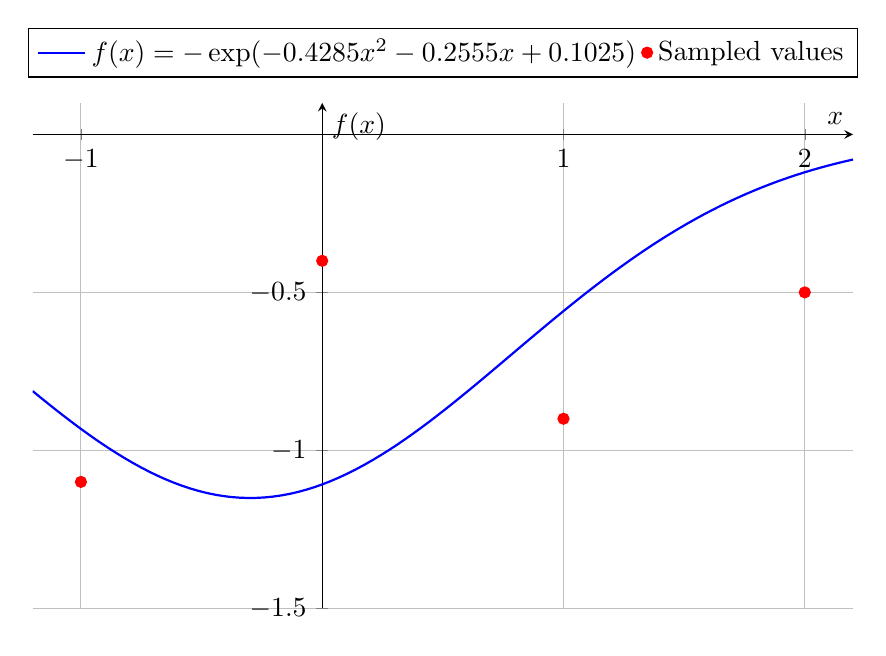
\begin{tikzpicture}
  \begin{axis}[
    domain=-1.2:2.2,
    samples=100,
    axis lines=middle,
    xlabel={$x$},
    ylabel={$f(x)$},
    ymin=-1.5, ymax=0.1,
    xtick={-1, 0, 1, 2},
    ytick={-1.5,-1,-0.5,0},
    grid=both,
    legend style={at={(0.5,1.05)}, anchor=south, legend columns=2},
    width=12cm, height=8cm
  ]

  % Plot the fitted curve
  \addplot [domain=-1.2:2.2, blue, thick] 
    {-exp(-0.4285*x^2 - 0.2555*x + 0.1025)};
  \addlegendentry{$f(x) = -\exp(-0.4285x^2 - 0.2555x + 0.1025)$}

  % Plot the sample points
  \addplot [only marks, red, mark=*] 
    coordinates {
      (-1, -1.1)
      (0, -0.4)
      (1, -0.9)
      (2, -0.5)
    };
  \addlegendentry{Sampled values}

  \end{axis}
\end{tikzpicture}

\pagebreak 

\begin{shaded}
    \textbf{(8)} Approximate the data with $f(x) \sim a \cos x + b \sin x$.


\begin{center}
\begin{tabular}{|c|c c c c c c c c c c c|}
\hline
$x$ & 0 & 1 & 2 & 3 & 4 & 5 & 6 & 7 & 8 & 9 & 10 \\
\hline
$y$ & 1.8 & 3.5 & 2.1 & -1.0 & -3.3 & -2.7 & 0.9 & 3.3 & 2.8 & -0.1 & -3.0 \\
\hline
\end{tabular}
\end{center}
\end{shaded}

There is no way to transform $f$ into a polynomial model (that I kwow of). So
let's brute-force this: 

\begin{align*}
    E = E(a, b) 
    &= \sum_{i=0}^n \left( y_i - f(x_i) \right)^2\\ 
    &=\sum_{i=0}^n \left( y_i - (a \cos x_i + b \sin x_i) \right)^2 \\ &=\sum_{i=0}^n \left( y_i - a \cos x_i - b \sin x_i \right)^2 \\ 
\end{align*}

Now, it is easy to see that 

\begin{equation*}
    \frac{\partial E}{\partial a} = 2 \sum_{i=0}^n(a \cos x_i + b \sin x_i -
    y_i) \cos x_i, \qquad \frac{\partial E}{\partial b} = 2\sum_{i=0}^n(a \cos
    x_i + b \sin x_i - y_i) \sin x_i
\end{equation*}

Equating both expressions to zero, one obtains the system: 

\begin{align*}
    &a \sum_{i=0}^n \cos^2 x_i + b \sum_{i=0}^n \sin x_i \cos x_i = \sum_{i=0}^n
    y_i \cos x_i \\ 
    &a \sum_{i=0}^n \cos x_i \sin x_i+ b \sum_{i=0}^n \sin^2 x_i = \sum_{i=0}^n
    y_i \sin x_i \\ 
\end{align*}

In other words, we readily obtain the system 

\begin{equation*}
    \begin{bmatrix} 
        \sum_{i=0}^n \cos^2 x_i & \sum_{i=0}^n \sin x_i \cos x_i & \sum_{i=0}^n
        y_i \cos x_i\\
        \sum_{i=0}^n \cos x_i \sin x_i & \sum_{i=0}^n \sin^2 x_i & \sum_{i=0}^n
        y_i \sin x_i
    \end{bmatrix} 
\end{equation*}

Suffices to evaluate these sums using a calculator and solving the system to 
obtain the coefficients $a, b$ which minimize the squared distances from 
the model to the set of data points.

\pagebreak 

\begin{shaded}
    \textbf{(9)} Consider Legendre's polynomials $\mathcal{P} :=
    \left\{ P_0, P_1, P_2 \right\} $ on $[-1, 1]$ given by 

    \begin{equation*}
        P_0(x) = 1, \qquad P_1(x) = x, \qquad P_2(x) = x^2 - 1 / 3
    \end{equation*}

    Verify that the set $\mathcal{P}$ is ortogonal.
\end{shaded}

The set $\mathcal{P}$ is ortogonal (in $[a, b]$) if and only if there is a weight function
$\omega$ such that 

\begin{equation*}
    \int_a^b \omega(x) P_k(x) P_j(x) ~ dx = \alpha_j \delta_{jk}, \qquad j = 0,
    1, 2
\end{equation*}

for some $\left\{ \alpha_0, \alpha_1, \alpha_2 \right\} $ all positive. In
particular, if $\alpha_0 = \alpha_1 = \alpha_2 = 1$, the set is ortonormal.
Now, consider that $\Omega(x) = 1$ is a weight function. It is easy to verify
that 

\begin{equation*}
    \int_{-1}^1 \Omega(x) P_j^2(x) ~ dx > 0
\end{equation*}

for $j = 0, 1, 2$. Now, $\int_{-1}^1 \Omega(x)P_0(x)P_1(x)~ dx = \int_{-1}^1 x ~
dx=
0$. Similarly, 

\begin{equation*}
    \int_{-1}^1 \Omega(x)P_0(x) P_2(x) ~ dx \int_{-1}^0 x^2 - 1 / 3 ~ dx =
    \frac{2}{3} - \frac{2}{3} = 0
\end{equation*}

Etc. This excercise is silly as it amounts to solving integrals.

\pagebreak 

\begin{shaded}
    \textbf{(10)} Determine the linear and quadratic approximations of $f(x) = e^x$ in the
    least squares sense using Legendre's polynomials in $[-1, 1]$.
\end{shaded}

Let $\Phi = \left\{ 1, x, x^2 - 1 / 3 \right\} $, and use $\phi_0, \phi_1,
\phi_2$ to refer to the elements in this set in the order I wrote them. We know
$\Phi$ to be ortogonal. 

(Linear approximation) There is a set of coefficients $a_0, a_1$ of 

\begin{equation*}
    P(x) = \sum_{k=0}^n a_k \phi_k(x)
\end{equation*}

which minimizes 

\begin{equation*}
    \int_{-1}^1 \left[ f(x) - P(x) \right]^2 ~ dx
\end{equation*}

Since $\Phi$ is ortonormal, we have 

\begin{equation*}
    a_j = \frac{1}{\alpha_j} \int_a^b f(x) \phi_j(x) ~ dx, \qquad j = 0, 1
\end{equation*}

Recall that

\begin{equation*}
    \alpha_0 = \int_{-1}^1 \phi_0^2(x) = 2, \qquad \alpha_1 = \int_{-1}^1 \phi_1^2(x) ~ dx =
    \frac{2}{3}, \qquad \alpha_2 = \int_{-1}^2 \phi_2^2(x) ~ dx = \frac{8}{45}
\end{equation*}

This readily gives the system of equations: 


\begin{align*}
a_0 &= \frac{1}{2} \int_{-1}^1 e^x \, dx = \frac{1}{2}(e - e^{-1}) \\
a_1 &= \frac{3}{2} \int_{-1}^1 x e^x \, dx = \frac{3}{2} \left[ e^{-1} + e^{-1} \right] = \frac{3 \cdot 2}{2e} = \frac{3}{e}
\end{align*}


Hence, the desired polynomial approximation of $f(x) = e^x$  on $[-1, 1]$ is:


\begin{equation*}
P(x) = \frac{1}{2}(e - e^{-1}) + \frac{3}{e} \cdot x
\end{equation*}

\begin{center}
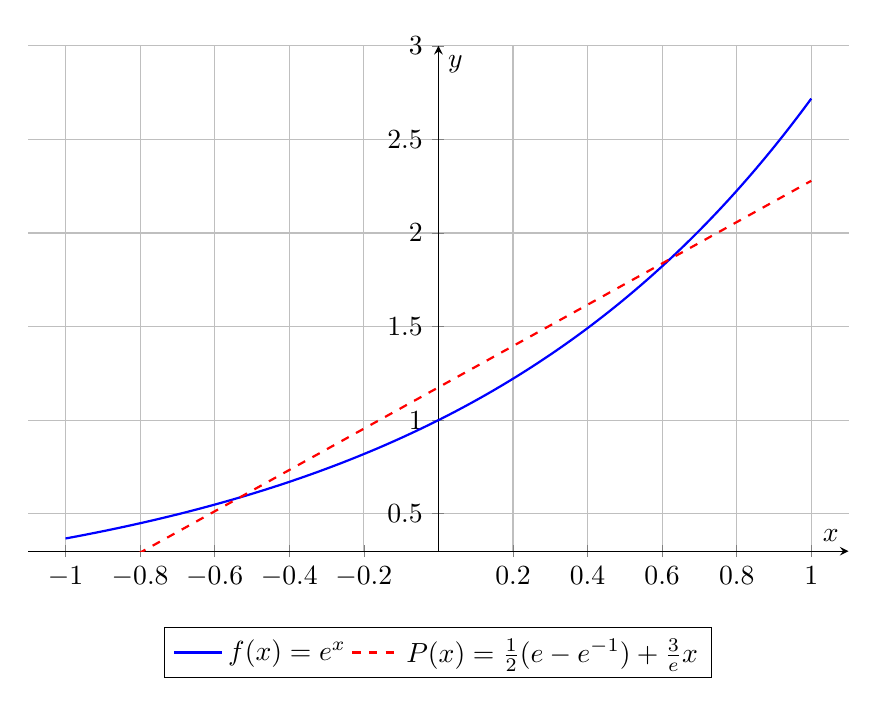
\begin{tikzpicture}
\begin{axis}[
    width=12cm,
    height=8cm,
    axis lines=middle,
    grid=major,
    xlabel={$x$},
    ylabel={$y$},
    xmin=-1.1, xmax=1.1,
    ymin=0.3, ymax=3,
    legend style={at={(0.5,-0.15)}, anchor=north, legend columns=2},
    domain=-1:1,
    samples=200
]
% Plot e^x
\addplot [blue, thick] {exp(x)};
\addlegendentry{$f(x) = e^x$}

% Plot linear approximation
\addplot [red, dashed, thick] {(1/2)*(exp(1) - 1/exp(1)) + (3/exp(1))*x};
\addlegendentry{$P(x) = \frac{1}{2}(e - e^{-1}) + \frac{3}{e}x$}
\end{axis}
\end{tikzpicture}
\end{center}

(Quadratic approximation) For a quadratic approximation, we now compute as well 

\begin{equation*}
    a_2 = \frac{45}{8} \int_{-1}^1 e^x(x^2 - 1 / 3) ~ dx = \frac{15(2e^2 - 14)}{8e}
\end{equation*}

So, the approximation is


\begin{equation*}
P(x) = \frac{1}{2}(e - e^{-1}) + \frac{3}{e} \cdot x + \frac{15(2e^2 -
14)}{8e}\left( x^2 - \frac{1}{3} \right) 
\end{equation*}


\begin{center}
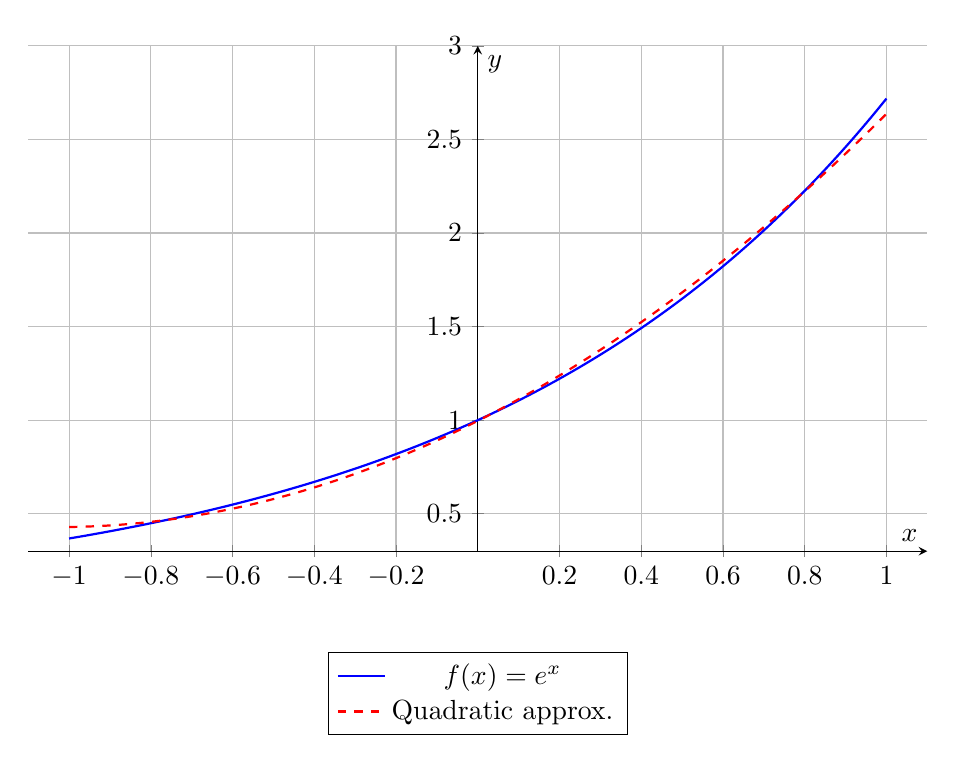
\begin{tikzpicture}
\begin{axis}[
    width=13cm,
    height=8cm,
    axis lines=middle,
    grid=major,
    xlabel={$x$},
    ylabel={$y$},
    xmin=-1.1, xmax=1.1,
    ymin=0.3, ymax=3,
    legend style={at={(0.5,-0.2)}, anchor=north, legend columns=1},
    domain=-1:1,
    samples=200
]
% f(x) = e^x
\addplot [blue, thick] {exp(x)};
\addlegendentry{$f(x) = e^x$}


% Quadratic approximation with phi_2 = x^2 - 1/3
\addplot [red, thick, dashed] {
    (1/2)*(exp(1) - 1/exp(1)) + 
    (3/exp(1))*x +
    ((30*exp(1) - 210/exp(1))/8)*(x^2 - 1/3)
};
\addlegendentry{Quadratic approx.}
\end{axis}
\end{tikzpicture}
\end{center}










\pagebreak 

\section{Numerical integration}

We'll estimate $\int_a^b f(x) ~ dx$ via $\sum_{i=0}^n a_i f(x_i)$, where 
$(x_0, y_0), \ldots, (x_n, y_n)$ are known values of $f$ (which itself might be
unknown) in the interval $[a, b]$. 

More generally, take $\left\{ x_i \right\}_{i=0}^n $ in $[a, b]$ and $P_n$ the
interpolating polynomial of $f$ in those nodes in Lagrange's form. Then we have 

\begin{equation*}
    P_n(x) = \sum_{i=0}^n f(x_i) \ell_i(x), \qquad e_n(x) =
    \frac{f^{(n+1)(\zeta_x)}}{(n+1)!} \eta_{n+1}(x)
\end{equation*}

for $\zeta_x \in (x_0, x_n)$. Using the fact that $f(x) = P_n(x) + e_n(x)$,

\begin{align*}
    \int_a^b f(x) ~ dx 
    &= \int_a^b P_n(x) ~ dx + \int_a^b e_n(x) ~ dx \\ 
    &= \int_a^b \sum_{i=0}^n f(x_i) \ell_i(x) ~ dx + \int_a^b
    \frac{f^{(n+1)(\zeta_x)}}{(n+1)!} \eta_{n+1}(x) ~ dx \\ 
    &= \sum_{i=0}^n a_i f(x_i) + \frac{1}{(n+1)!}\int_a^b f^{(n+1)}(\zeta_x)
    eta_{n+1}(x) ~ dx
\end{align*}

from $\zeta_x \in (x_0, x_n)$ and $a_i = \int_a^b \ell_i(x) ~ dx$, $i = 0,
\ldots, n$.

\begin{equation}
    \therefore ~ \int_a^b f(x) ~ dx \approx \sum_{i=0}^n a_i f(x_i)
\end{equation}

with an error 

\begin{equation}
    E_n(f) = \frac{1}{(n+1)!}\int_a^b f^{(n+1)}(\zeta_x) \eta_{n+1}(x) ~ dx
\end{equation}

\subsection{Trapeze rule}

Trapeze's rule is the name for the case $n = 1$ (linear integration). By
convention, $x_0 = a, x_1 = b, h = b- a$. The interpolating polynomial es 

\begin{equation*}
    P_1(x) = \frac{x-x_1}{x_0 - x_1} f(x_0) + \frac{x-x_0}{x_1 - x_0} f(x_1)
\end{equation*}

with error 

\begin{equation*}
    e_1(x) = \frac{f''(\zeta_x)}{2!}(x-x_0)(x-x_1)
\end{equation*}

Simplifying equation $(1)$ for this case, 

\begin{align*}
    \int_a^b f(x) ~ dx &\approx f(x_0)\int_a^b \frac{x-x_1}{x_0 - x_1} ~ dx +
    f(x_1) \int_a^b \frac{x-x_0}{x_1 - x_0} ~ dx \\ 
    &= \frac{h}{2}\left( f(a) + f(b) \right) 
\end{align*}

To simplify the expression of the error, the following theorem is used. 

\begin{theorem}[Pretty theorem]
    Assume $f \in C[a,b]$ and $g$ integrable and either always positive or
    always negative in $[a, b]$. Then there is some $c \in (a, b)$ such that 

    \begin{equation*}
        \int_a^b f(x) g(x)~ dx = f(c) \int_a^b g(x) ~ dx
    \end{equation*}

    If $g(x) \equiv 1$ then $\int_a^b f(x) ~ dx = f(c)(b-a)$, entailing that 

    \begin{equation*}
        f(c) = \frac{1}{b-a}\int_a^b f(x) ~ dx
    \end{equation*}
\end{theorem}

It is easy to see that $(x - x_0)(x-x_1)$ satisfies the conditions of the
theorem, meaning that there is some $\zeta$ (independent of $x$) such that 

\begin{align*}
    \int_a^b (\zeta_x)(x-a)(x-b) ~ dx 
    &= f''(\zeta)\int_a^b(x-a)(x-b) ~ dx\\ 
    &= f''(\zeta)\left[ \frac{x^3}{3} - \frac{a+b}{2} x^2 + abx \right]_a^b
\end{align*}





















\end{document}











